\documentclass[conference]{IEEEtran}
\IEEEoverridecommandlockouts
% The preceding line is only needed to identify funding in the first footnote. If that is unneeded, please comment it out.
\usepackage{cite}
\usepackage{amsmath,amssymb,amsfonts}
\usepackage{algorithmic}
\usepackage{graphicx}
\usepackage{textcomp}
\usepackage{xcolor}
\usepackage{url}
\usepackage{subcaption}


\def\BibTeX{{\rm B\kern-.05em{\sc i\kern-.025em b}\kern-.08em
    T\kern-.1667em\lower.7ex\hbox{E}\kern-.125emX}}
\begin{document}

\title{DICOMViz  \\ \LARGE Python based Dicom Images Visualizer}

\author{\IEEEauthorblockN{Pablo Giaccaglia}
\IEEEauthorblockA{\textit{Politecnico di Milano} \\
pablo.giaccaglia@mail.polimi.it}
}

\maketitle
\begin{abstract}
In this report we analyze \textit{DICOMViz}, a modular, expandable and lightweight portable DICOM viewer application written in Python and Qt. It allows to load and view Dicom series, single acquisitions and their tag data. The supported medical images, such as Computed Radiography (CR), Computed Tomography (CT) and Magnetic Resonance Imaging (MRI) images, can be exported in different formats, copied to clipboard, viewed as animations in case of series, rotated, zoomed in and out and examined with other utilities. Even though the current state of the application is not oriented to image processing, additional features allow to operate with negative colors images, color maps, exposure, lungs masks and segmentation. The UI, written in the renowned QT Framework Python binding Pyqt, plays an important role, ensuring a fluent and user friendly interaction thanks to a simple but customizable layout.
\end{abstract}

\begin{IEEEkeywords}
Dicom, Python, Qt
\end{IEEEkeywords}

\section{Introduction}\
DICOM (Digital Imaging and Communications in Medicine)\cite{b1} is the international standard format for viewing, store and share medical images, along with patient and acquisition details. This information is stored inside a DICOM image file and can be viewed through specific software solutions that can read and display the format. The standard, whose first release was in 1983, has become predominant among medical students and professionals, since it is implemented in almost every radiology, cardiology imaging, and radiotherapy device. Every day thousands of DICOM images are exchanged, viewed and stored for clinical care, through the use of a multitude of viewing software options. The huge interest and development in this field among the years has lead to the availability of hundreds of software solutions, from the research oriented one to the business solution, such as  \textit{RadiAnt}\cite{b2} and  \textit{PostDICOM}\cite{b3}. Each of these has different specifications, system requirements, plug-ins and capabilities and target different users' needs. Starting from the operating system, many viewers are designed to run on either Windows or Mac, but not both. Some viewers support multiple devices, allowing to access the same data from desktops, tables and smartphones interchangeably. Finally the main intention when using such software plays an important role in the choice process. Medical students usually look for a simple viewer to study clinical images like CT, MRI and ultrasound. On the other hand clinician may be looking for more advanced tools to analyze specific body regions and work with image processing features like maximum and minimum intensity projections and 3D reconstruction.


\section{Proposed work}
In the context of Dicom software solutions, where the abundance can make the choice difficult, the DICOMViz application is proposed. The aim of this project is to provide a simple and lightweight cross-platform Python application mainly meant for basic viewing, developed with the intention of exploring the capabilities of the DICOM standard through the  \textit{PyDicom} Python package\cite{b5}, whose results are visually shown through a user-friendly and intuitive interface, providing a single toolbar with only a few but useful tools, which can be quickly learned. Another goal of this project, which allowed to implement the above mentioned interface, is to show how simple and effective is the integration of the standard images with several powerful Python libraries, which resulted in a totally modular, maintainable and extensible application. The core tools and libraries are now listed, briefly described
and their use motivated:

\begin{itemize}
    \item \textbf{Pydicom\cite{b5}}: this is the core package used by the application, a pure Python package for working with DICOM files (.dcm extension). By wrapping the standard, this library can run anywhere Python runs without any other requirements, allowing to read, modify and write DICOM data through "pythonic" data structures and easy manipulation routines.

    \item \textbf{NumPy \cite{b6}}: since \textbf{Pydicom} is not primarily intended for viewing images, pixel data extracted from files has to be properly handled through other tools like this one. Moreover the application relies on the  \textit{Qt} Framework and the  \textit{PyQtGraph} library, built on top of  \textit{PyQt}, this is why the need of operating with  \textit{NumPy} arrays is mandatory. This package has also been used to execute fast pixel data manipulations such as rotations and flips, bit-wise inversion for negative images or masks, lung segmentation creation in case of lungs acquisitions.

    \item \textbf{Qt Designer\cite{b7}}: a  \textit{Qt} Framework tool which helps in the GUI building process, through a  \textit{Rapid Application Development} (RAD) approach, allowing to operate with Qt Widgets in a graphical way, following a  "\textit{What You See Is What You Get}" (WYSIWYG) process. Windows can be composed with Widgets and customized following application needs and the result can be translated to fully functional  \textit{PyQt} code.

    \item \textbf{PyQt \cite{b8}}: one of the most popular Python bindings for the Qt cross-platform C++ Framework. The binding adopted for this application is  \textit{PyQt6}, which supports Qt version 6 and runs on all platforms supported by Qt, including Windows, macOS and Linux.
    Its use in DicomViz is essential, since it allows to work with the generated Qt Designer code, as a starting point for the interface development through Qt Widgets (UI primary elements), and with the  \textit{PyQtGraph} library for interactive fast imaging display. In the rest of the paper, when a Qt Widget is mentioned, the actual referred element is a  \textit{PyQtWidget}.

    \item \textbf{PyQtGraph\cite{b9}}: as mentioned above, this is a Python library built on top of  \textit{PyQt}, providing high performance graphics and numerical calculations support, thanks to Qt’s  \textit{GraphicsView} Framework and  \textit{Numpy}. This library finds its place within DicomViz in the actual image visualization, thanks to the utilities provided by the  \textit{ImageView} PyQtGraph Widget, such as scaling, exposure levels and histogram manipulations, color map choice and real time playback of image sequences.
\end{itemize}

Due to the modular and highly customizable nature of the used UI libraries, several static adaptations and, when obtaining custom behaviours without modifications of library source code was impossible, monkey patches were implemented to improve usability and to obtain a captivating interface. Further details about this are provided in the following sections.
In the next section a brief overview of the implemented features is provided, to have a clearer vision of the application capabilities and of the effective impact of the above listed libraries.

\section{Implemented Functionalities}

The modular approach of the underlying architecture backing up DicomViz is reflected also in the user interface, whose various sections' (\textit{Qt Widgets}) descriptions are the right starting point to understand application's capabilities. Their names and descriptions are here listed:

\begin{itemize}
    \item \textbf{Main Window}: a  \textit{QtMainWindow} subclass providing the main window application as a container of  \textit{QWidgets}. It is the component to instantiate as an entry point to DicomViz when running a  \textit{QApplication}. All the following components are added to its layout.

    \item \textbf{Menu Bar}: a  \textit{QMenuBar} subclass representing the only horizontal menu bar of the application, providing various functionalities through pull down menu items. This interface component  automatically sets its own geometry to the top of the " \textit{Main Windo}" and changes it appropriately whenever the aforementioned is resized.

    \item \textbf{DICOM View}: a PyQtGraph  \textit{ImageView} subclass providing functions to show the  \textit{NumPy} array pixel data, zoom in and out, rotate, change exposure and color maps, export, copy to clipboard and more.

    \item \textbf{DICOM Tags}: a  \textit{QTreeView} subclass to show DICOM header data in a tree-like structure, where for each tag and subtag the name, the tag identifier and the field value are shown. This section is dynamically updated each time a different image is loaded into the " \textit{DICOM View}".

    \item \textbf{Docks}: " \textit{Dicom Dock Files}" and " \textit{Dicom Dock Series}" are the 2 subclasses of  \textit{QDockWidget} representing utility windows which can be moved inside the " \textit{Main Window}" by the user according to its needs. The role of these components is to store in a vertical list structure the file names of images not belonging to a series for the former dock, of series' images for the latter dock. These lists are interactive and the click of one element causes the corresponding image to be shown in the " \textit{DICOM View}" section. In the case of the series' dock file names are shown in a sorted ordering, according to the " \textit{Slice Location}" tag field, to ensure a scrolling experience coherent with the physical acquisition sequence.

    \item \textbf{Series}: a  \textit{QTableView} subclass providing a sortable list of currently loaded series with some related information, such as the number of images, the patient's name and the series UID. This list is interactive, provides a search-by-word functionality and the click of one element causes the " \textit{Dicom Dock Series}" content to be filled with series' images file names and the " \textit{Dicom View}" section to show the first image of the series.

\end{itemize}

In the following subsections various implemented functionalities are described and the interaction between the various QT's  \textit{QWidgets} explained above is shown.

\subsection{Dynamic UI}

With the goal of keeping interface layout simple and partially customizable at run time, the application let the user change the occupied space of various components and, in the case of the 2 dock windows showing both the list of single files and  \textit{Dicom Series} images, to place them in different locations inside the UI's main window. The purpose of this feature is to address different type of user's needs during the utilization experience, by allowing the user to decide the right space to assign to each element according to the particular operation performed. For example a user could be interested only in viewing an image, so the hiding of the other components is possible thanks to the resizable PyQt  \textit{splitters} defining the layout borders. Another possible scenario sees an user interested only in viewing  \textit{Dicom Series} images metadata, visible in the " \textit{DICOM Tags}" box, while scrolling through the various files listed in the " \textit{Dicom Dock Series}". The freedom given to the user is only partial, since the intention is to provide a flexible experience without leading the user to to get lost in the customization.

 \begin{figure}[h]
    \begin{minipage}{.49\columnwidth}
        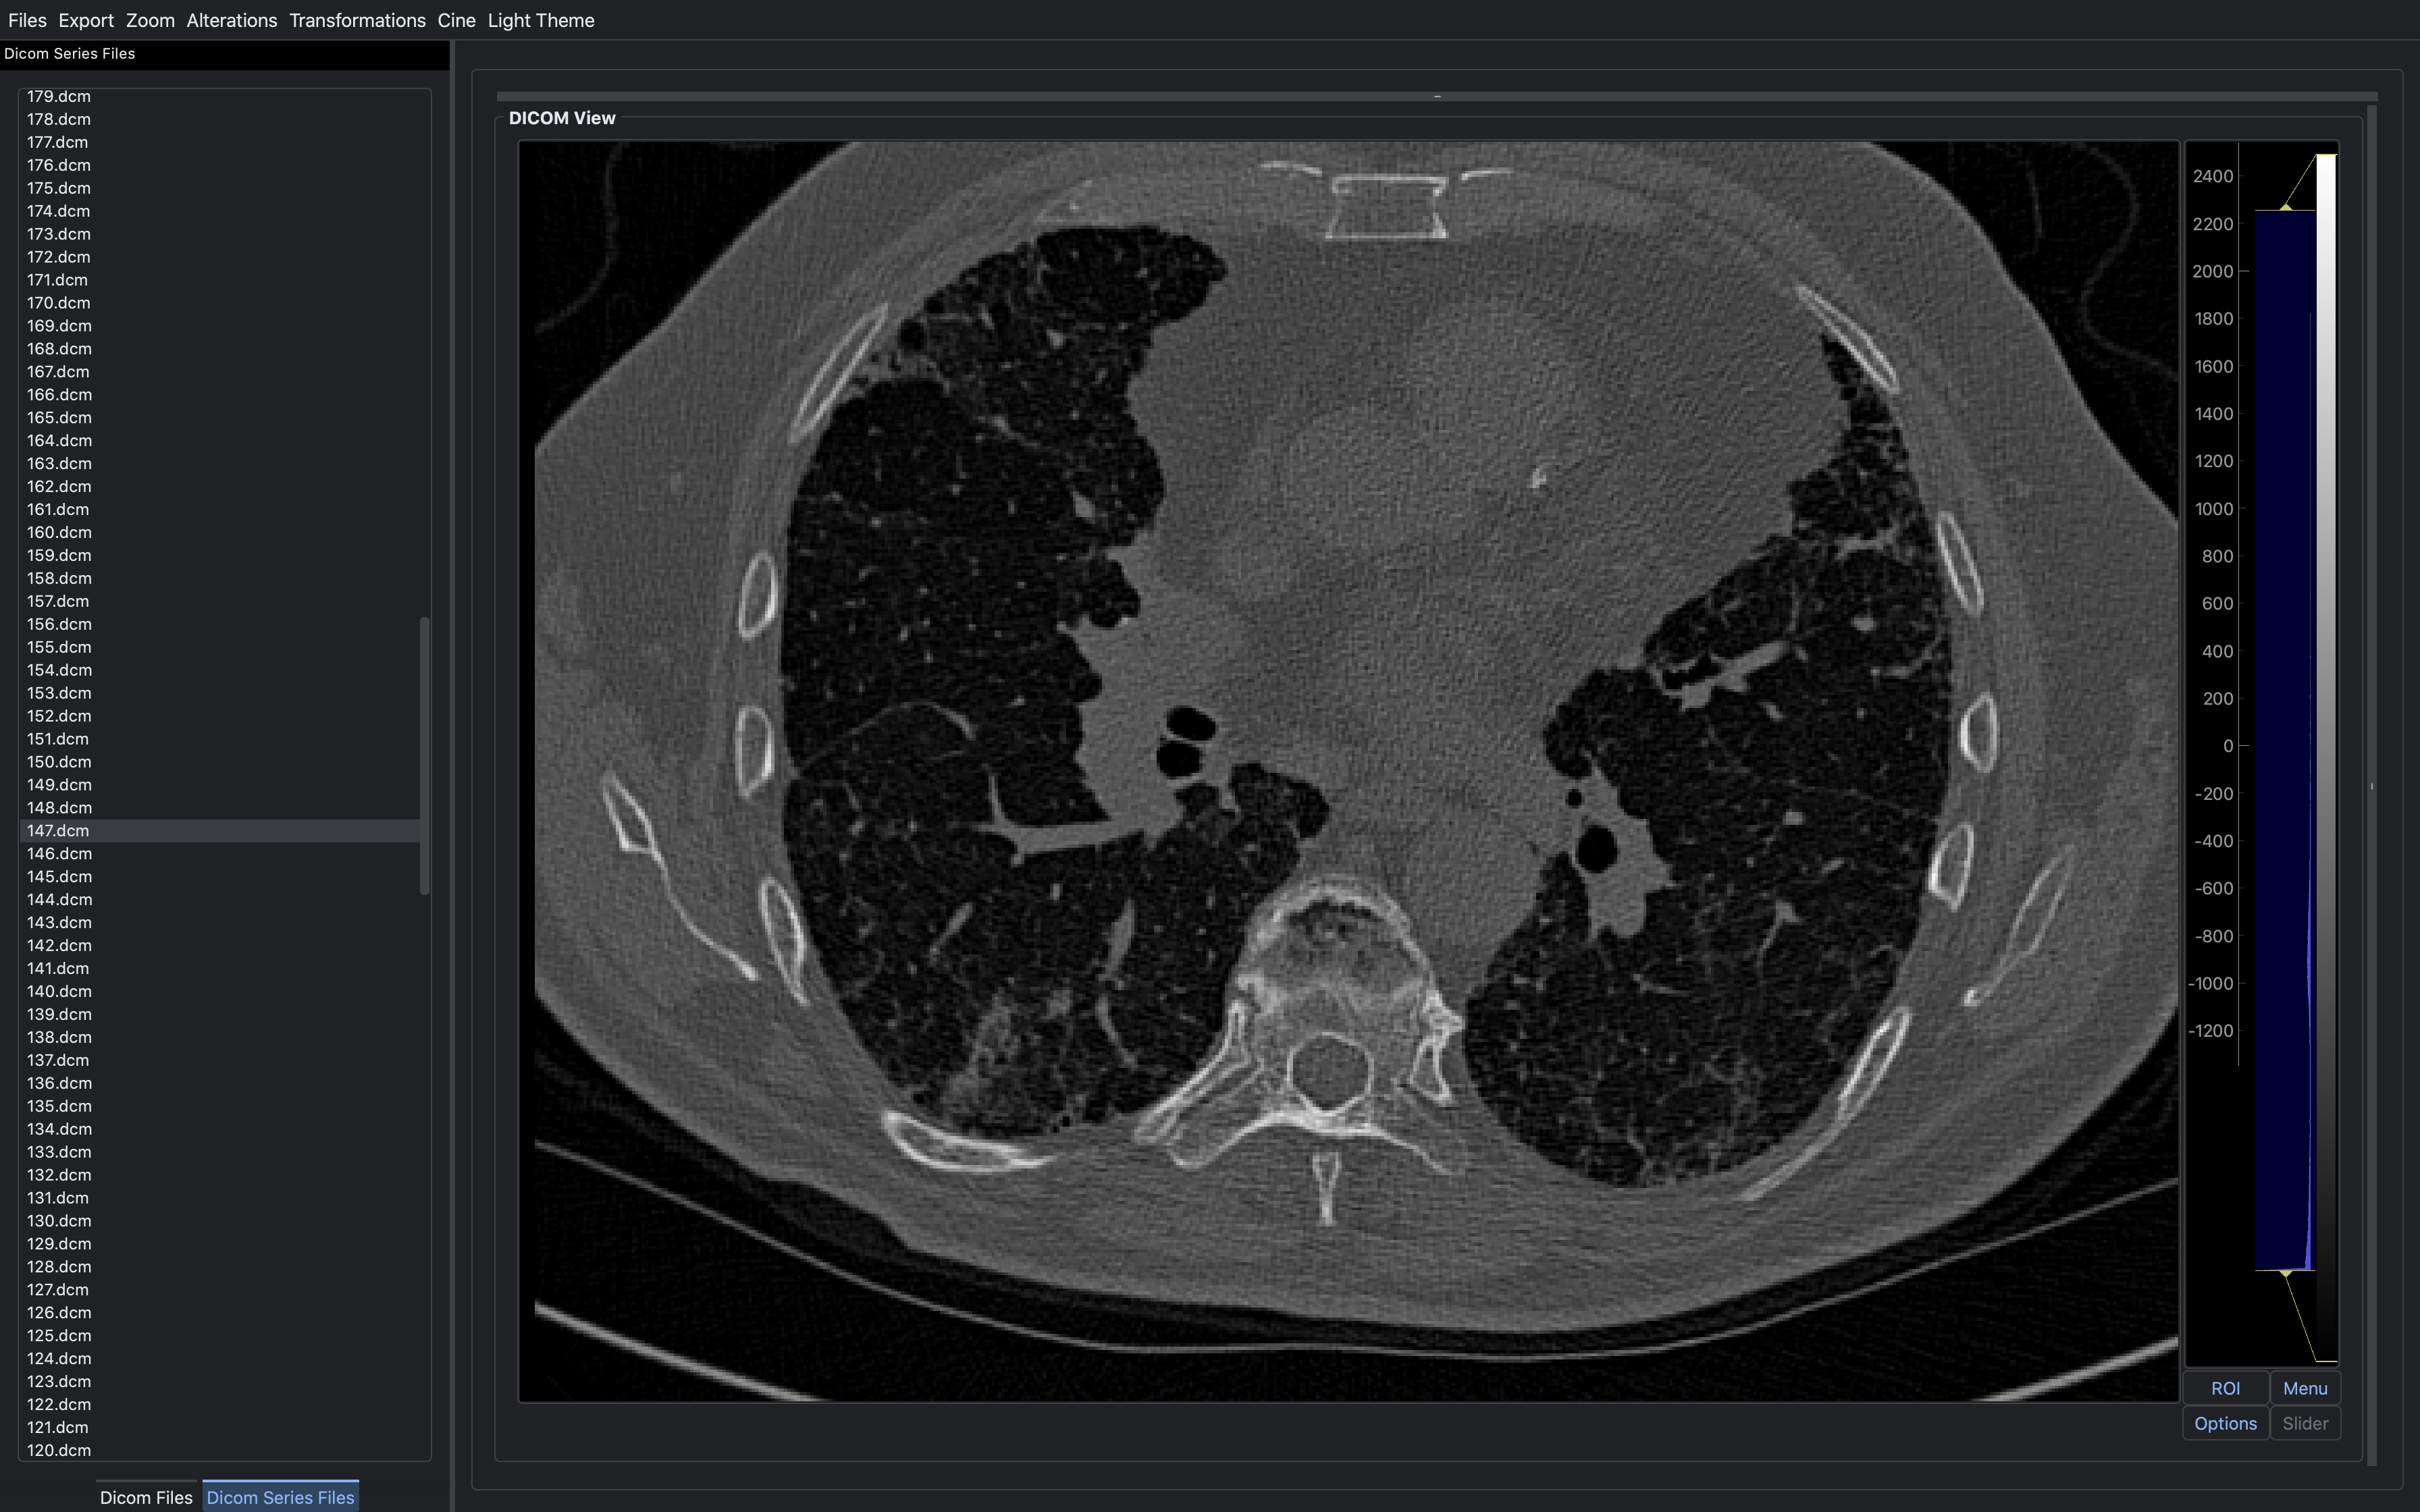
\includegraphics[width=\columnwidth]{image focus.png}
        \subcaption{}
    \end{minipage}\hfill
    \begin{minipage}{.49\columnwidth}
        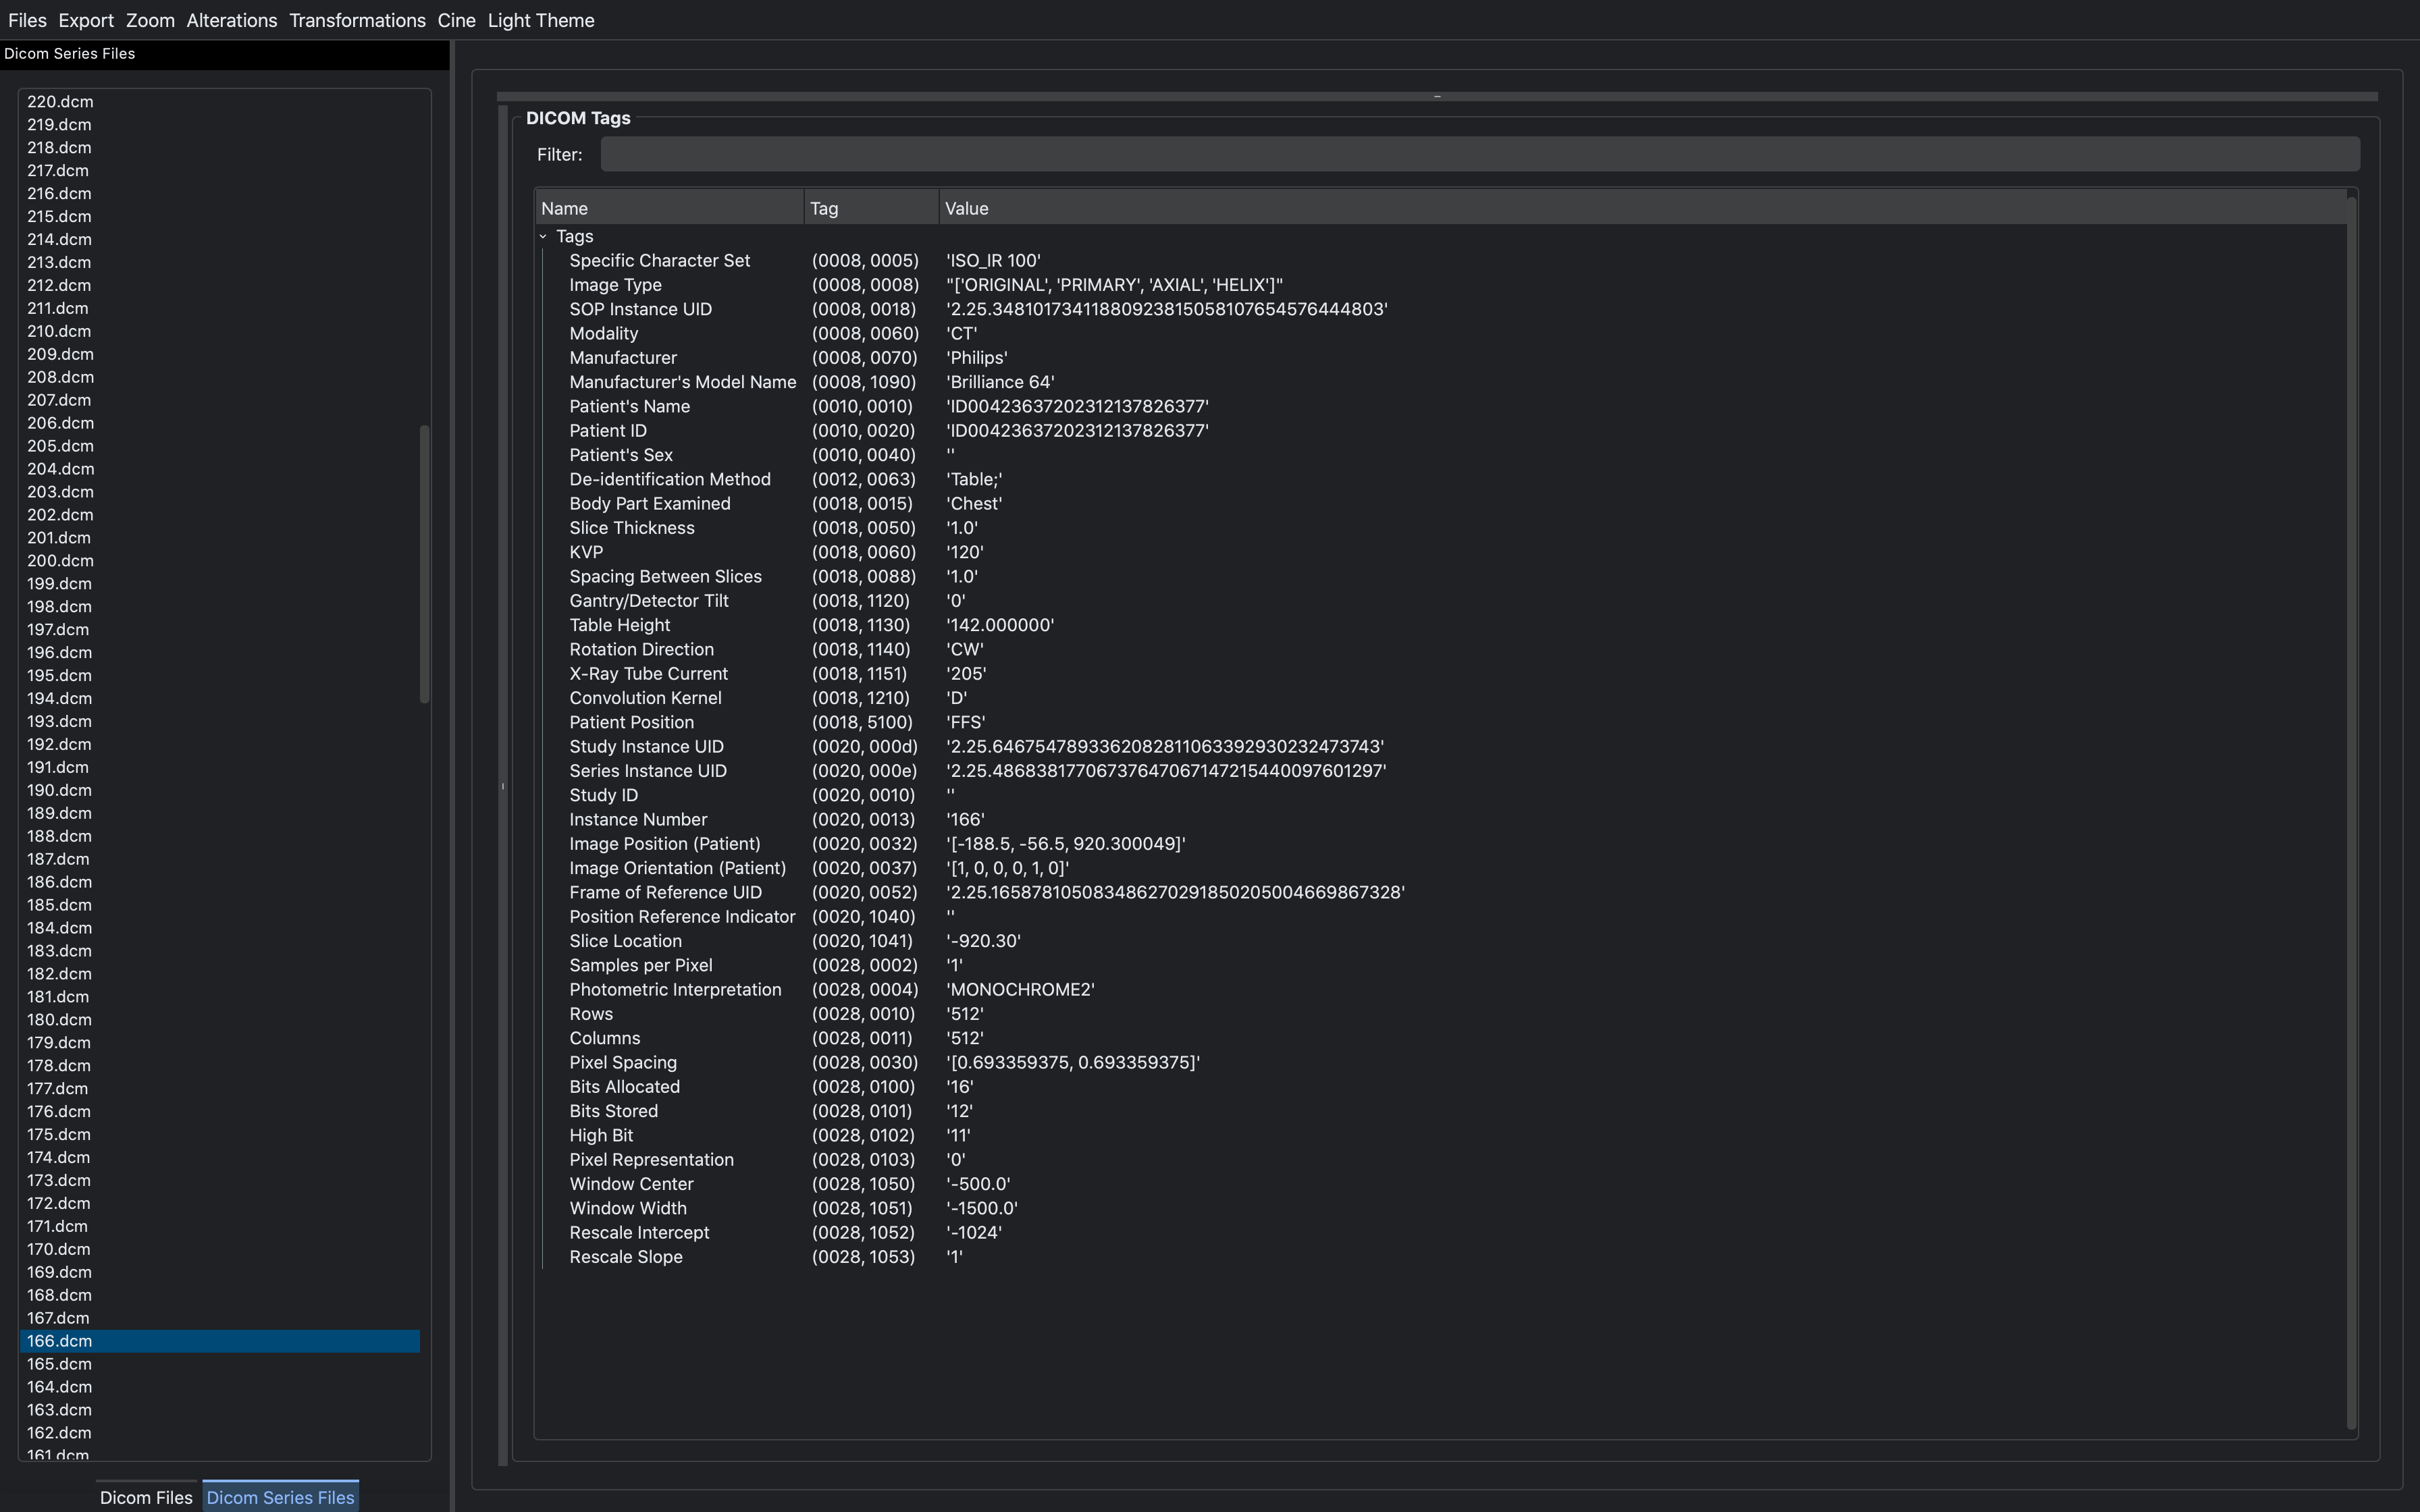
\includegraphics[width=\columnwidth]
        {tags focus.png}
        \subcaption{}
    \end{minipage}
    \caption{\tiny (a) shows the scenario in which the user customizes the layout to focus on the shown Dicom image, while (b) shows the scenario in which the user focuses on Dicom files and their corresponding tags}
\end{figure}

\subsection{Image Visualization}

As previously explained, the "\textit{DICOM View}" component is the delegated one to show images on screen. Thanks to the several functionalities provided by  \textit{PyQtGraph}, the image viewing is enriched with some basic but powerful options, which can highlight certain image features if properly combined together. Apart from the already mentioned zoom, color maps and exposure functionalities, further tweaks include background color change, translations, region of interest ( \textit{ROI}) plots, automatic histogram fitting the view, automatic image fitting the view and automatic optimal exposure.
When a new image has to be set to view, what the  \textit{ImageView} subclass receives as input is a  \textit{NumPy} array representing the Dicom pixel data, extracted from the field " \textit{pixel\_array}" of the corresponding  \textit{PyDicom} structure, called " \textit{Dataset}". The previously cited alterations, such as lungs segmentation, are shown through this component as a final result, but the necessary pixel manipulation process is done through custom functions external to the  \textit{PyQtGraph} module and explained in the section "\textit{Image Alterations}".

\begin{figure}[h]
  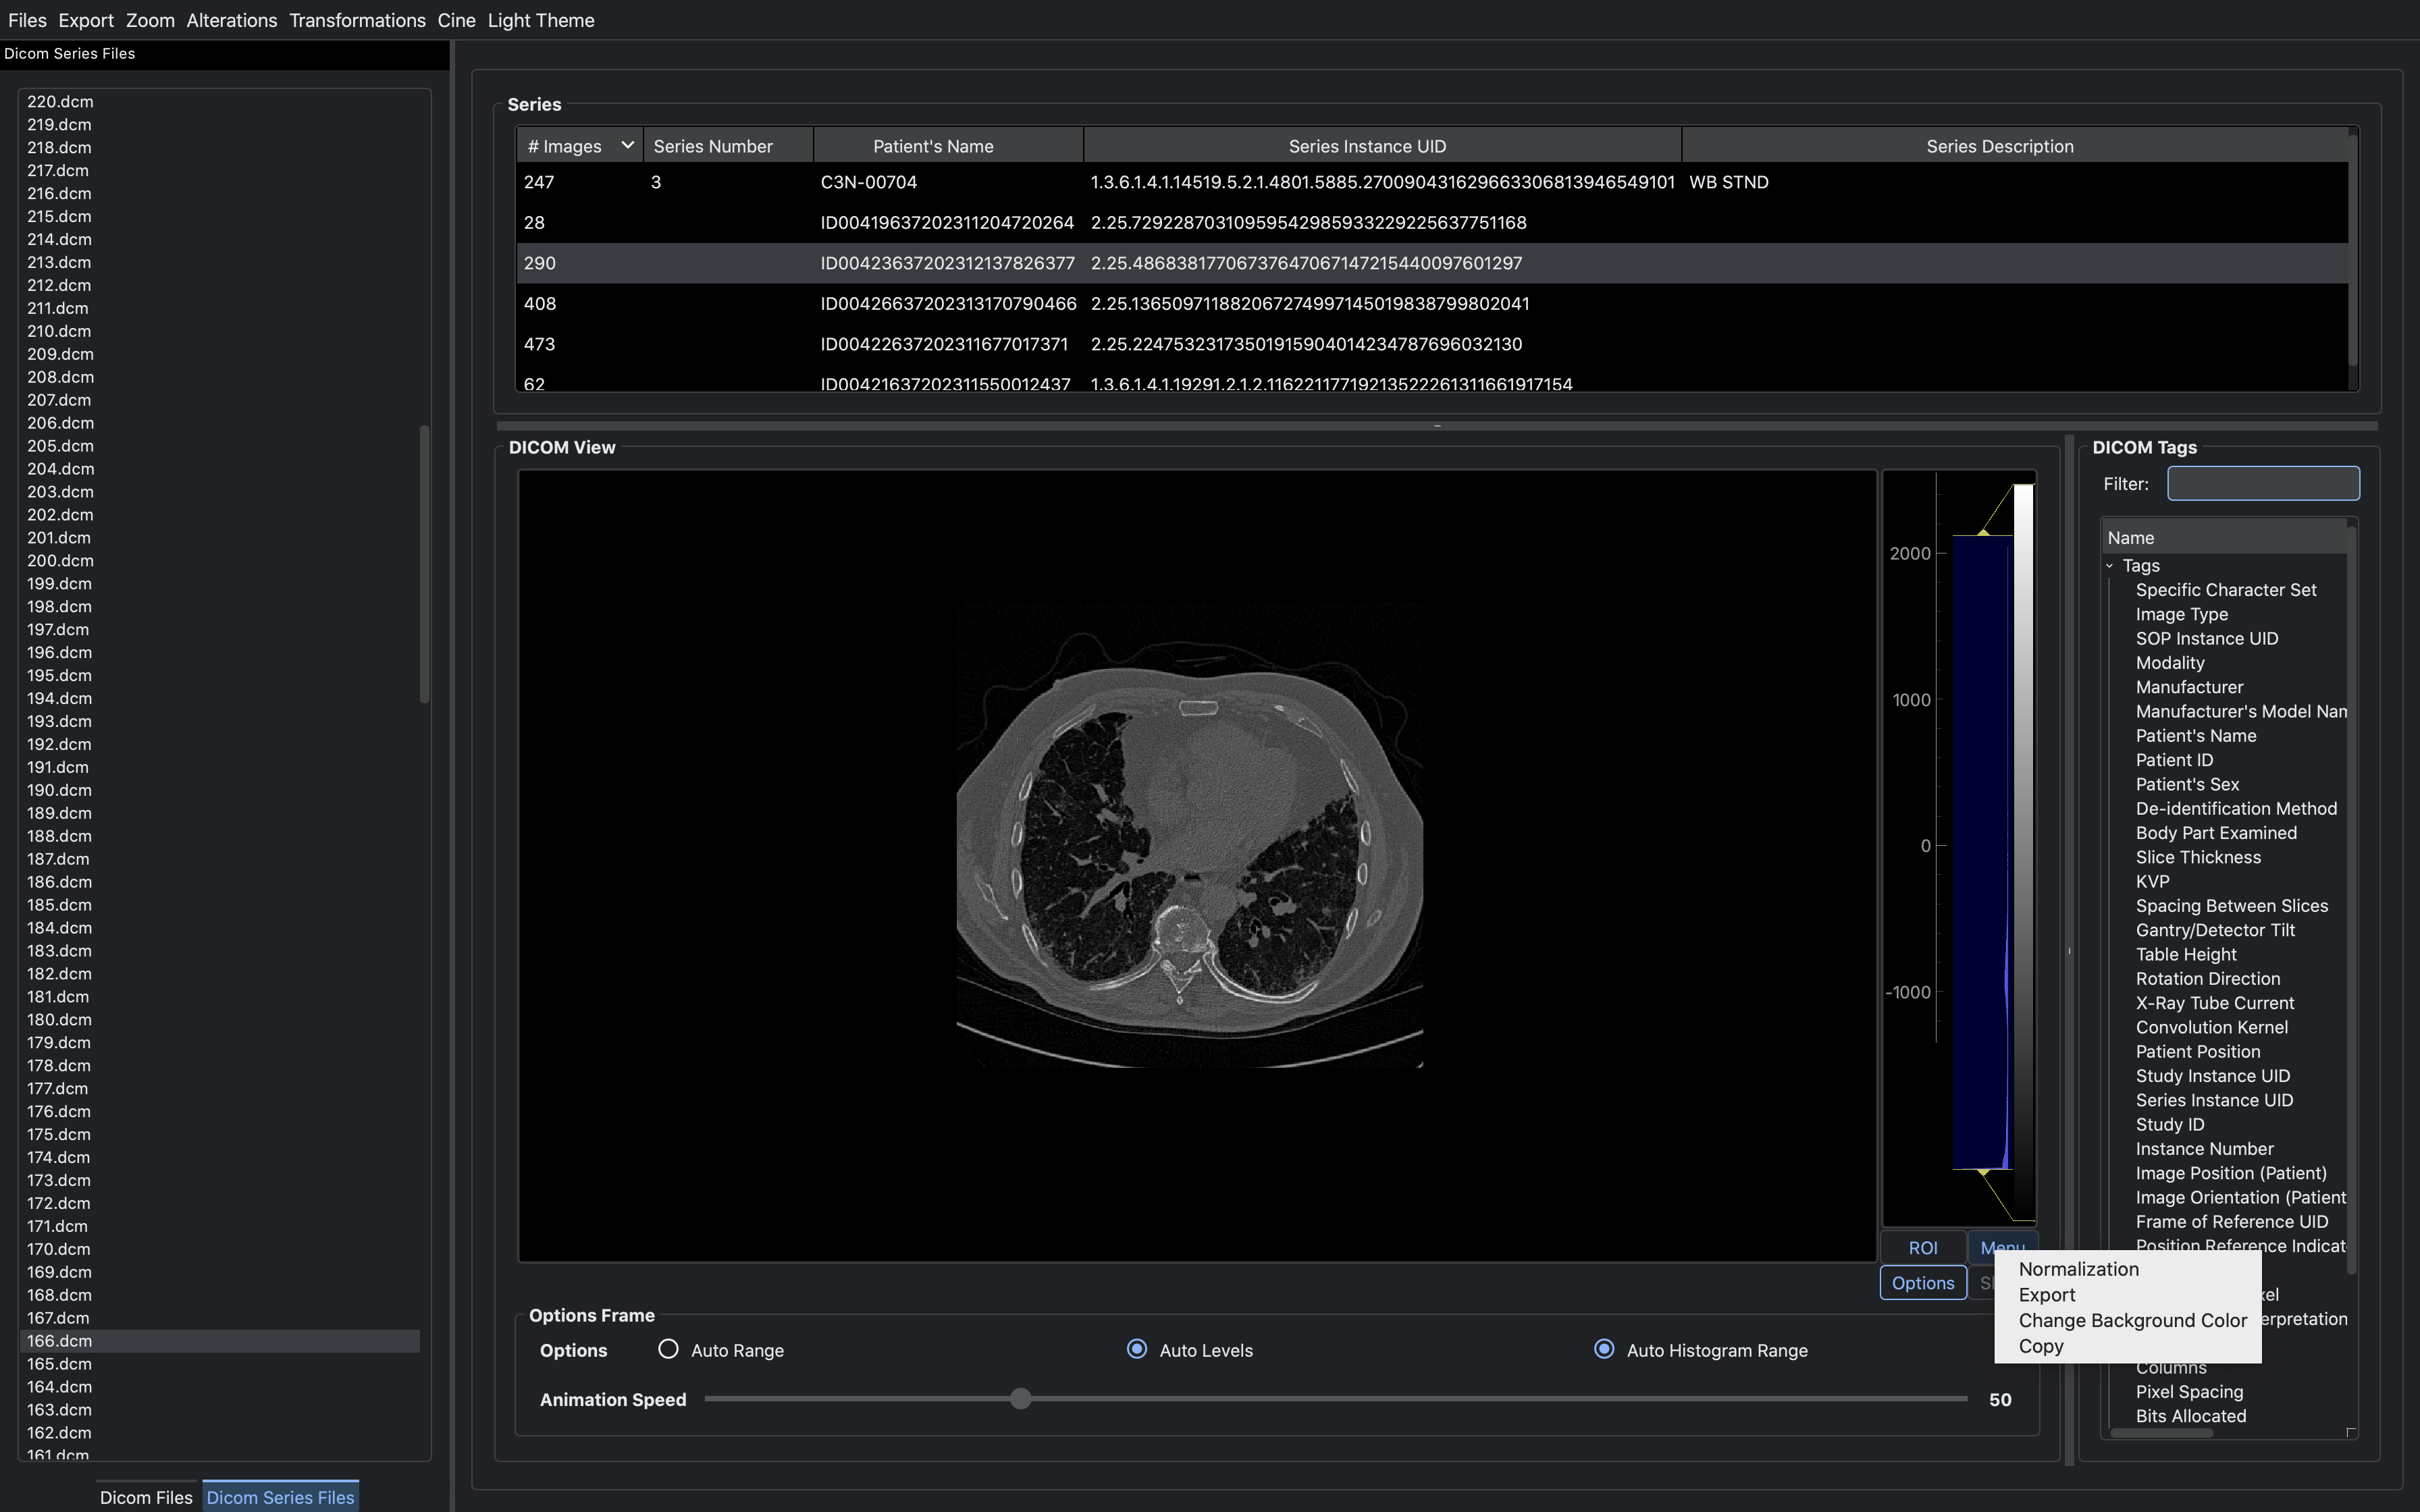
\includegraphics[width=\columnwidth]
    {overall.png}\hfill
  \caption{The figure shows an example of a possible view, in which the " \textit{Options Frame}" is set visible, showing various toggable options and a disabled slider, usable for series animation speed control}
\end{figure}


\subsection{Series Visualization}

A Dicom series is handled by DicomViz through a custom data structure called "DicomSeries", which is created if in the imported folder of Dicom files is found a sequence of images having and sharing the same  \textit{Series UID}. Then the "Series" TreeView is filled with the proper information and the "Dock Series View" is populated with the corresponding file names. Finally the first image of the series is selected, shown on the "Image View" and its tags are reported on the "DICOM Tags" section. When working with series, in addition to the enabled functionalities shared with non-series belonging files, described in the previous subsection, animation and gif export functionalities are enabled and will be explained in the following sections.

\subsection{Export}

The exporting of files is made possible thanks to the exporter object provided by the  \textit{PyQtGraph} Export Dialog, accessible natively by right clicking on the shown image or on the ROI plot. There are various available exporting options.
When working with images, some of these options include PNG, JPEG, TIFF, ICO and SVG.
When working with plots apart from the already mentioned, more formats are available, which are CSV and HDF5.
Through monkey patching the images export dialog is made available in 2 additional locations of the UI.
The first additional "Export" option is available within the pull down menu accessible by clicking the "Menu" button, located in the "\textit{DICOM View}" section.
The second additional " \textit{Export}" option is available within the "Export" " \textit{MenuBar}" entry, by clicking in the " \textit{Export File}" button.

\begin{figure}[h]
  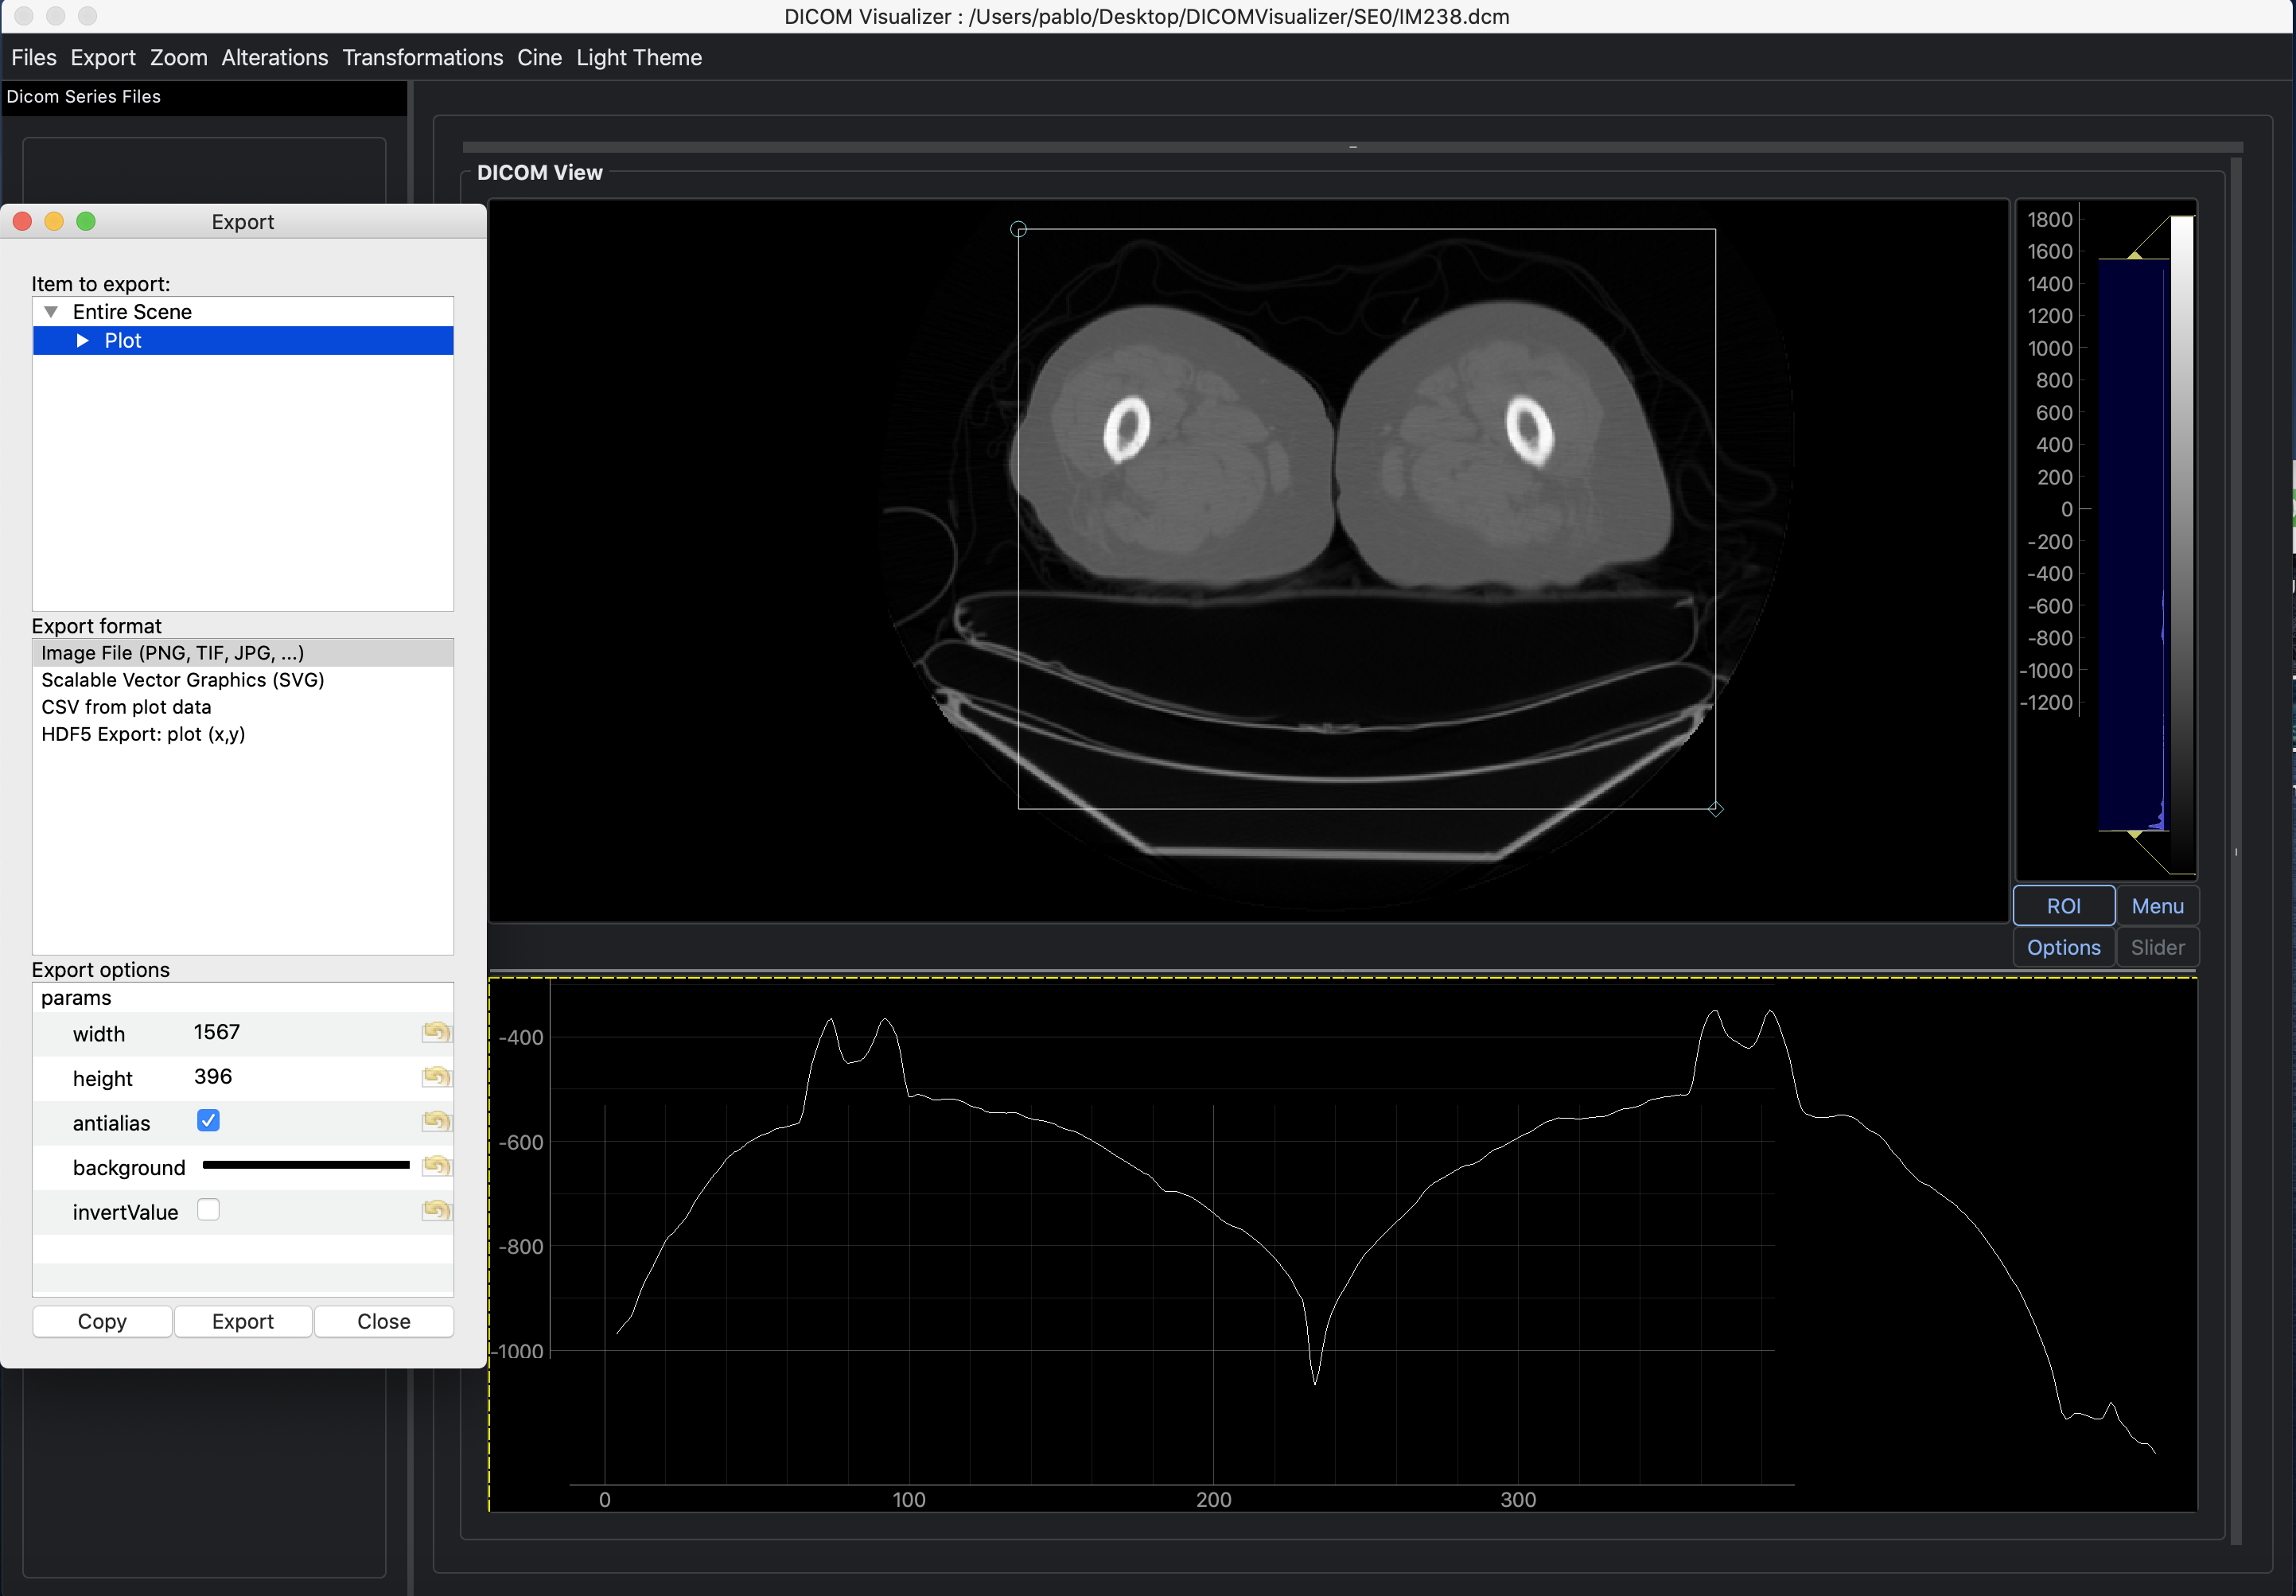
\includegraphics[width=\columnwidth]
    {export.png}\hfill
  \caption{Export dialog of a ROI plot}
\end{figure}

\subsection{Animation \& GIF Export}

An important difference between single files and series within DicomViz is that the latter allows to play animated visualizations. This feature is made possible thanks to the  \textit{QTimer} class, which provides a high-level, multithreaded environment compliant interface for system timers , allowing to have a fluent alternation of shown images in a non-blocking way, with respect to the "\textit{Main Window}". The animation is handled through a custom QWidget, called  \textit{AnimationHandler}, which also supports dynamic speed changes of the shown images. The speed value can be changed during animation by the user through the "\textit{Animation Speed}" slider, available within the " \textit{Options Frame}" in the "\textit{DICOM View}" UI section. When working with series it is also made possible to export animation GIF files of the whole sequence, thanks to a custom Exporter, called " \textit{GifExporter}", added at runtime to the ExportDialog, since it is not included natively in the  \textit{PyQtGraph} library.

\begin{figure*}[h]
        \begin{subfigure}[b]{0.475\textwidth}
            \centering
            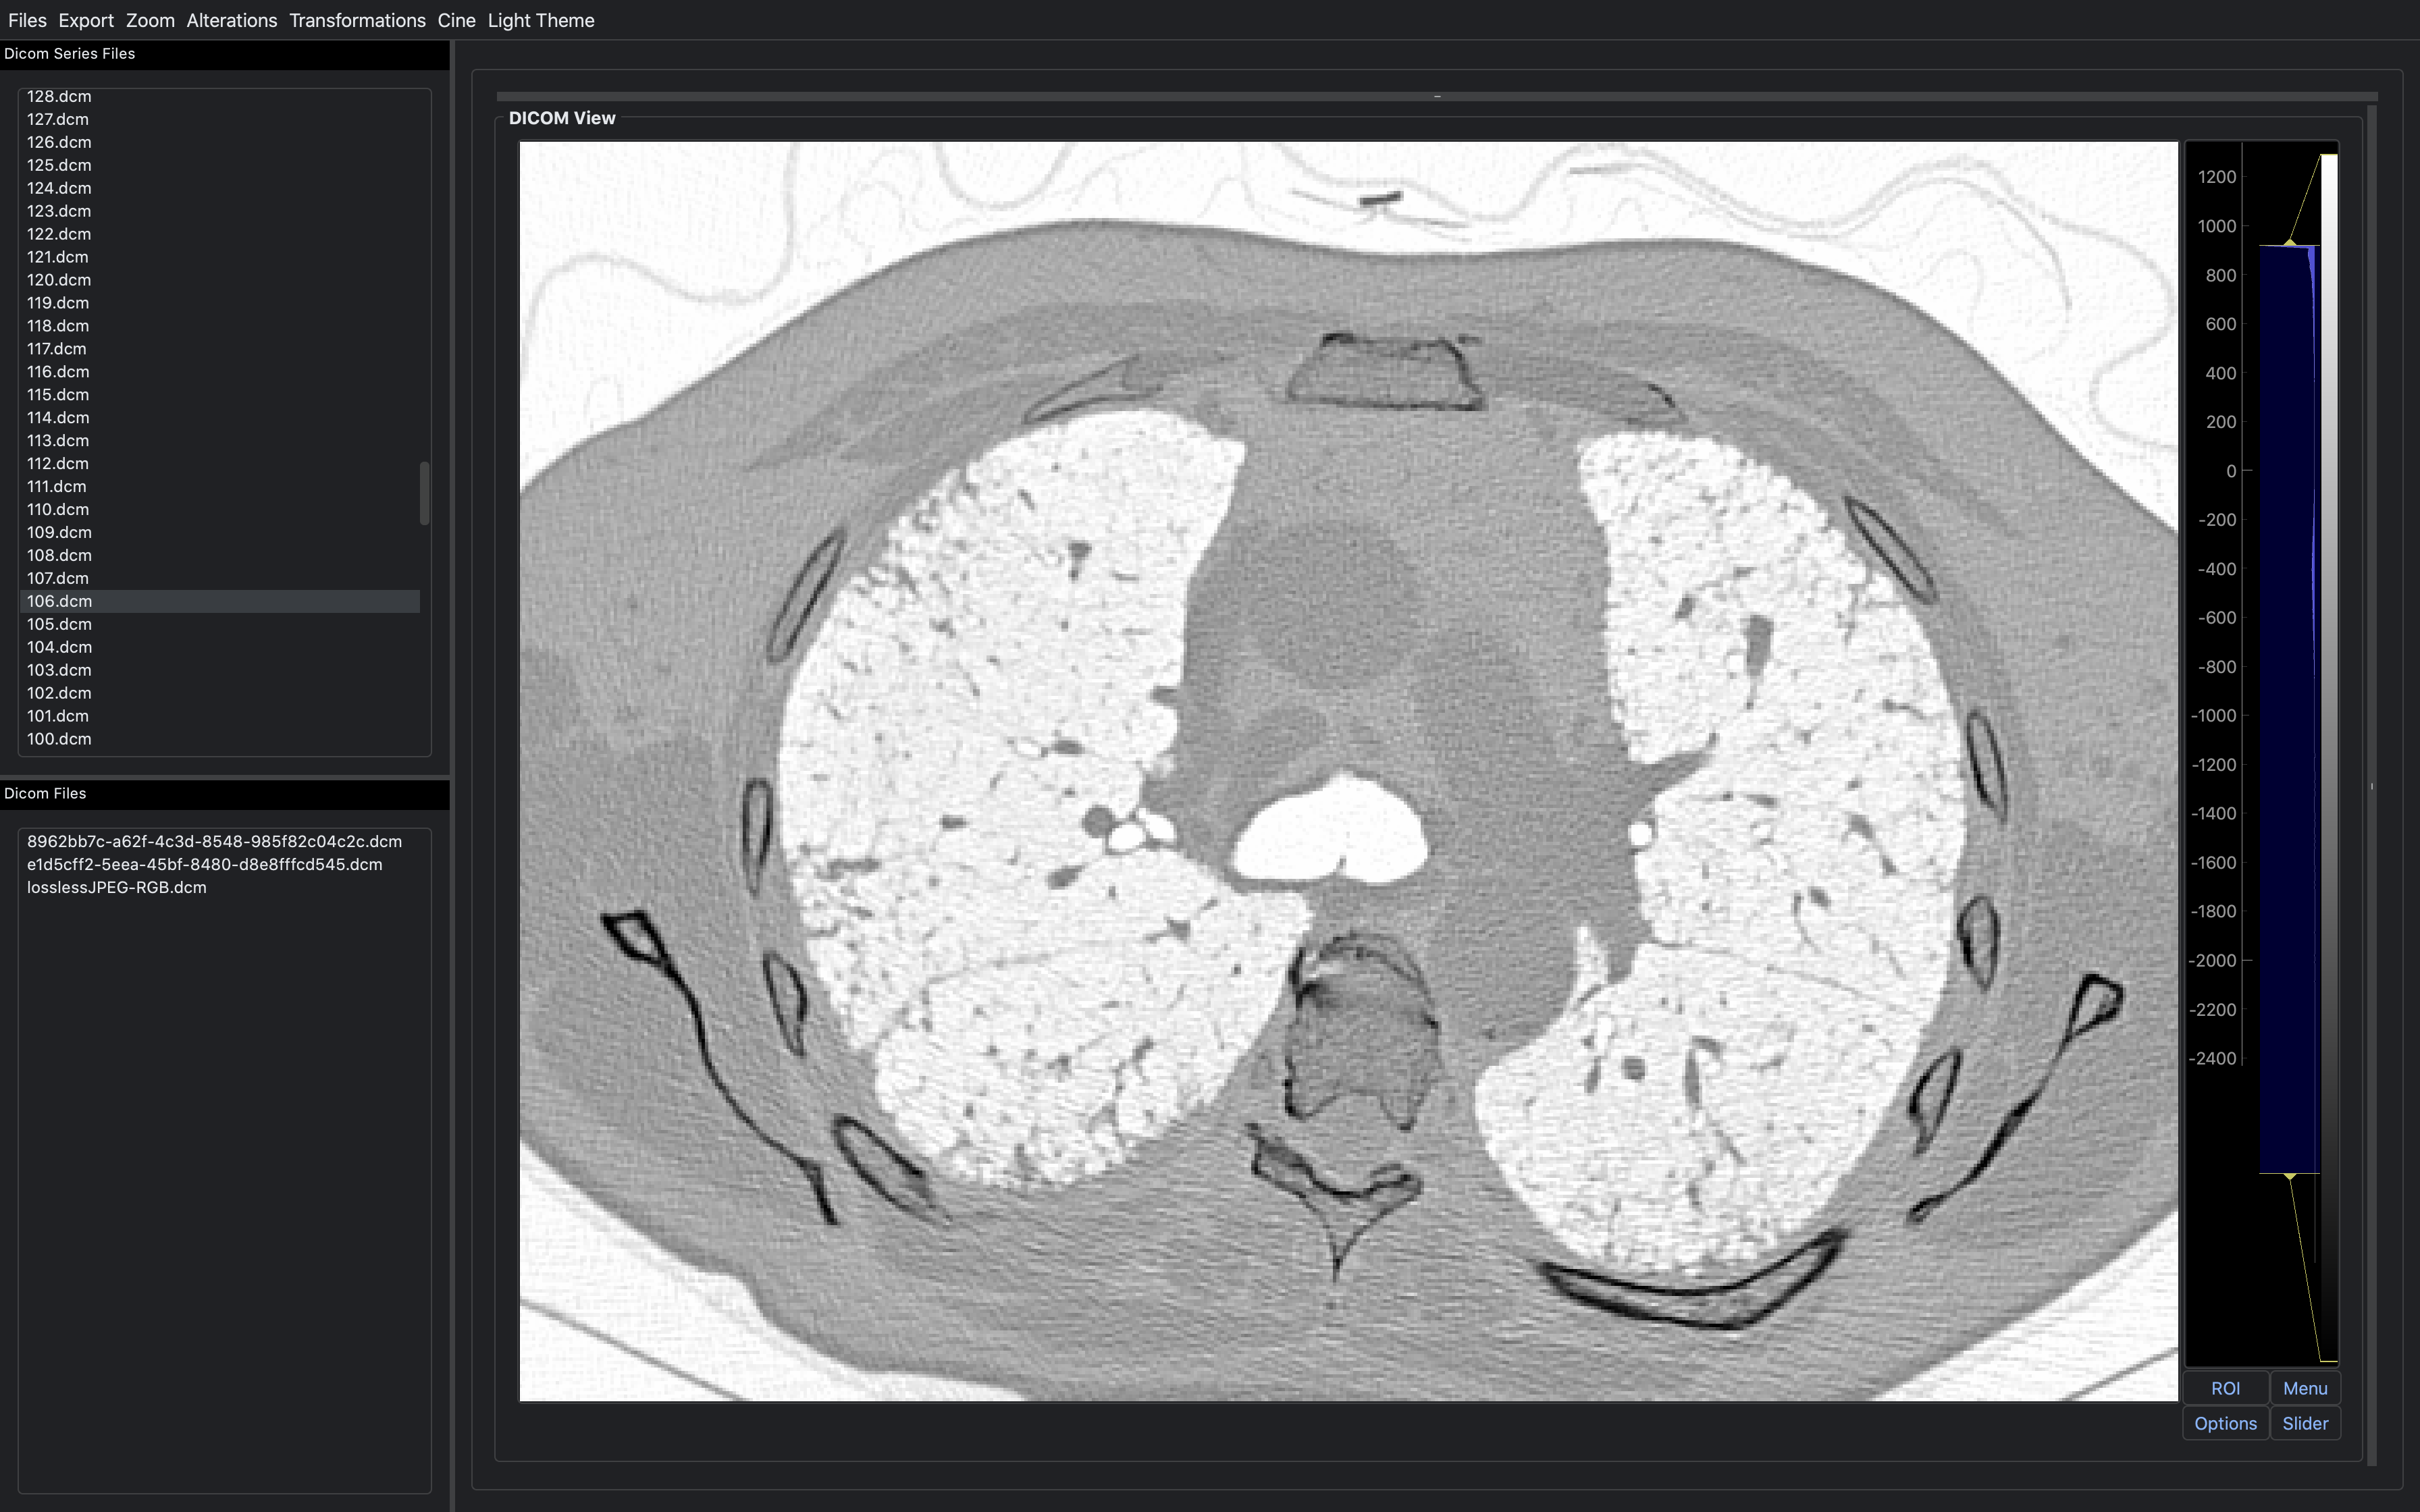
\includegraphics[width=\textwidth]{negative2.png}
            \caption[]%
            {{\small Negative image}}
            \label{fig:mean and std of net14}
        \end{subfigure}
        \hfill
        \begin{subfigure}[b]{0.475\textwidth}
            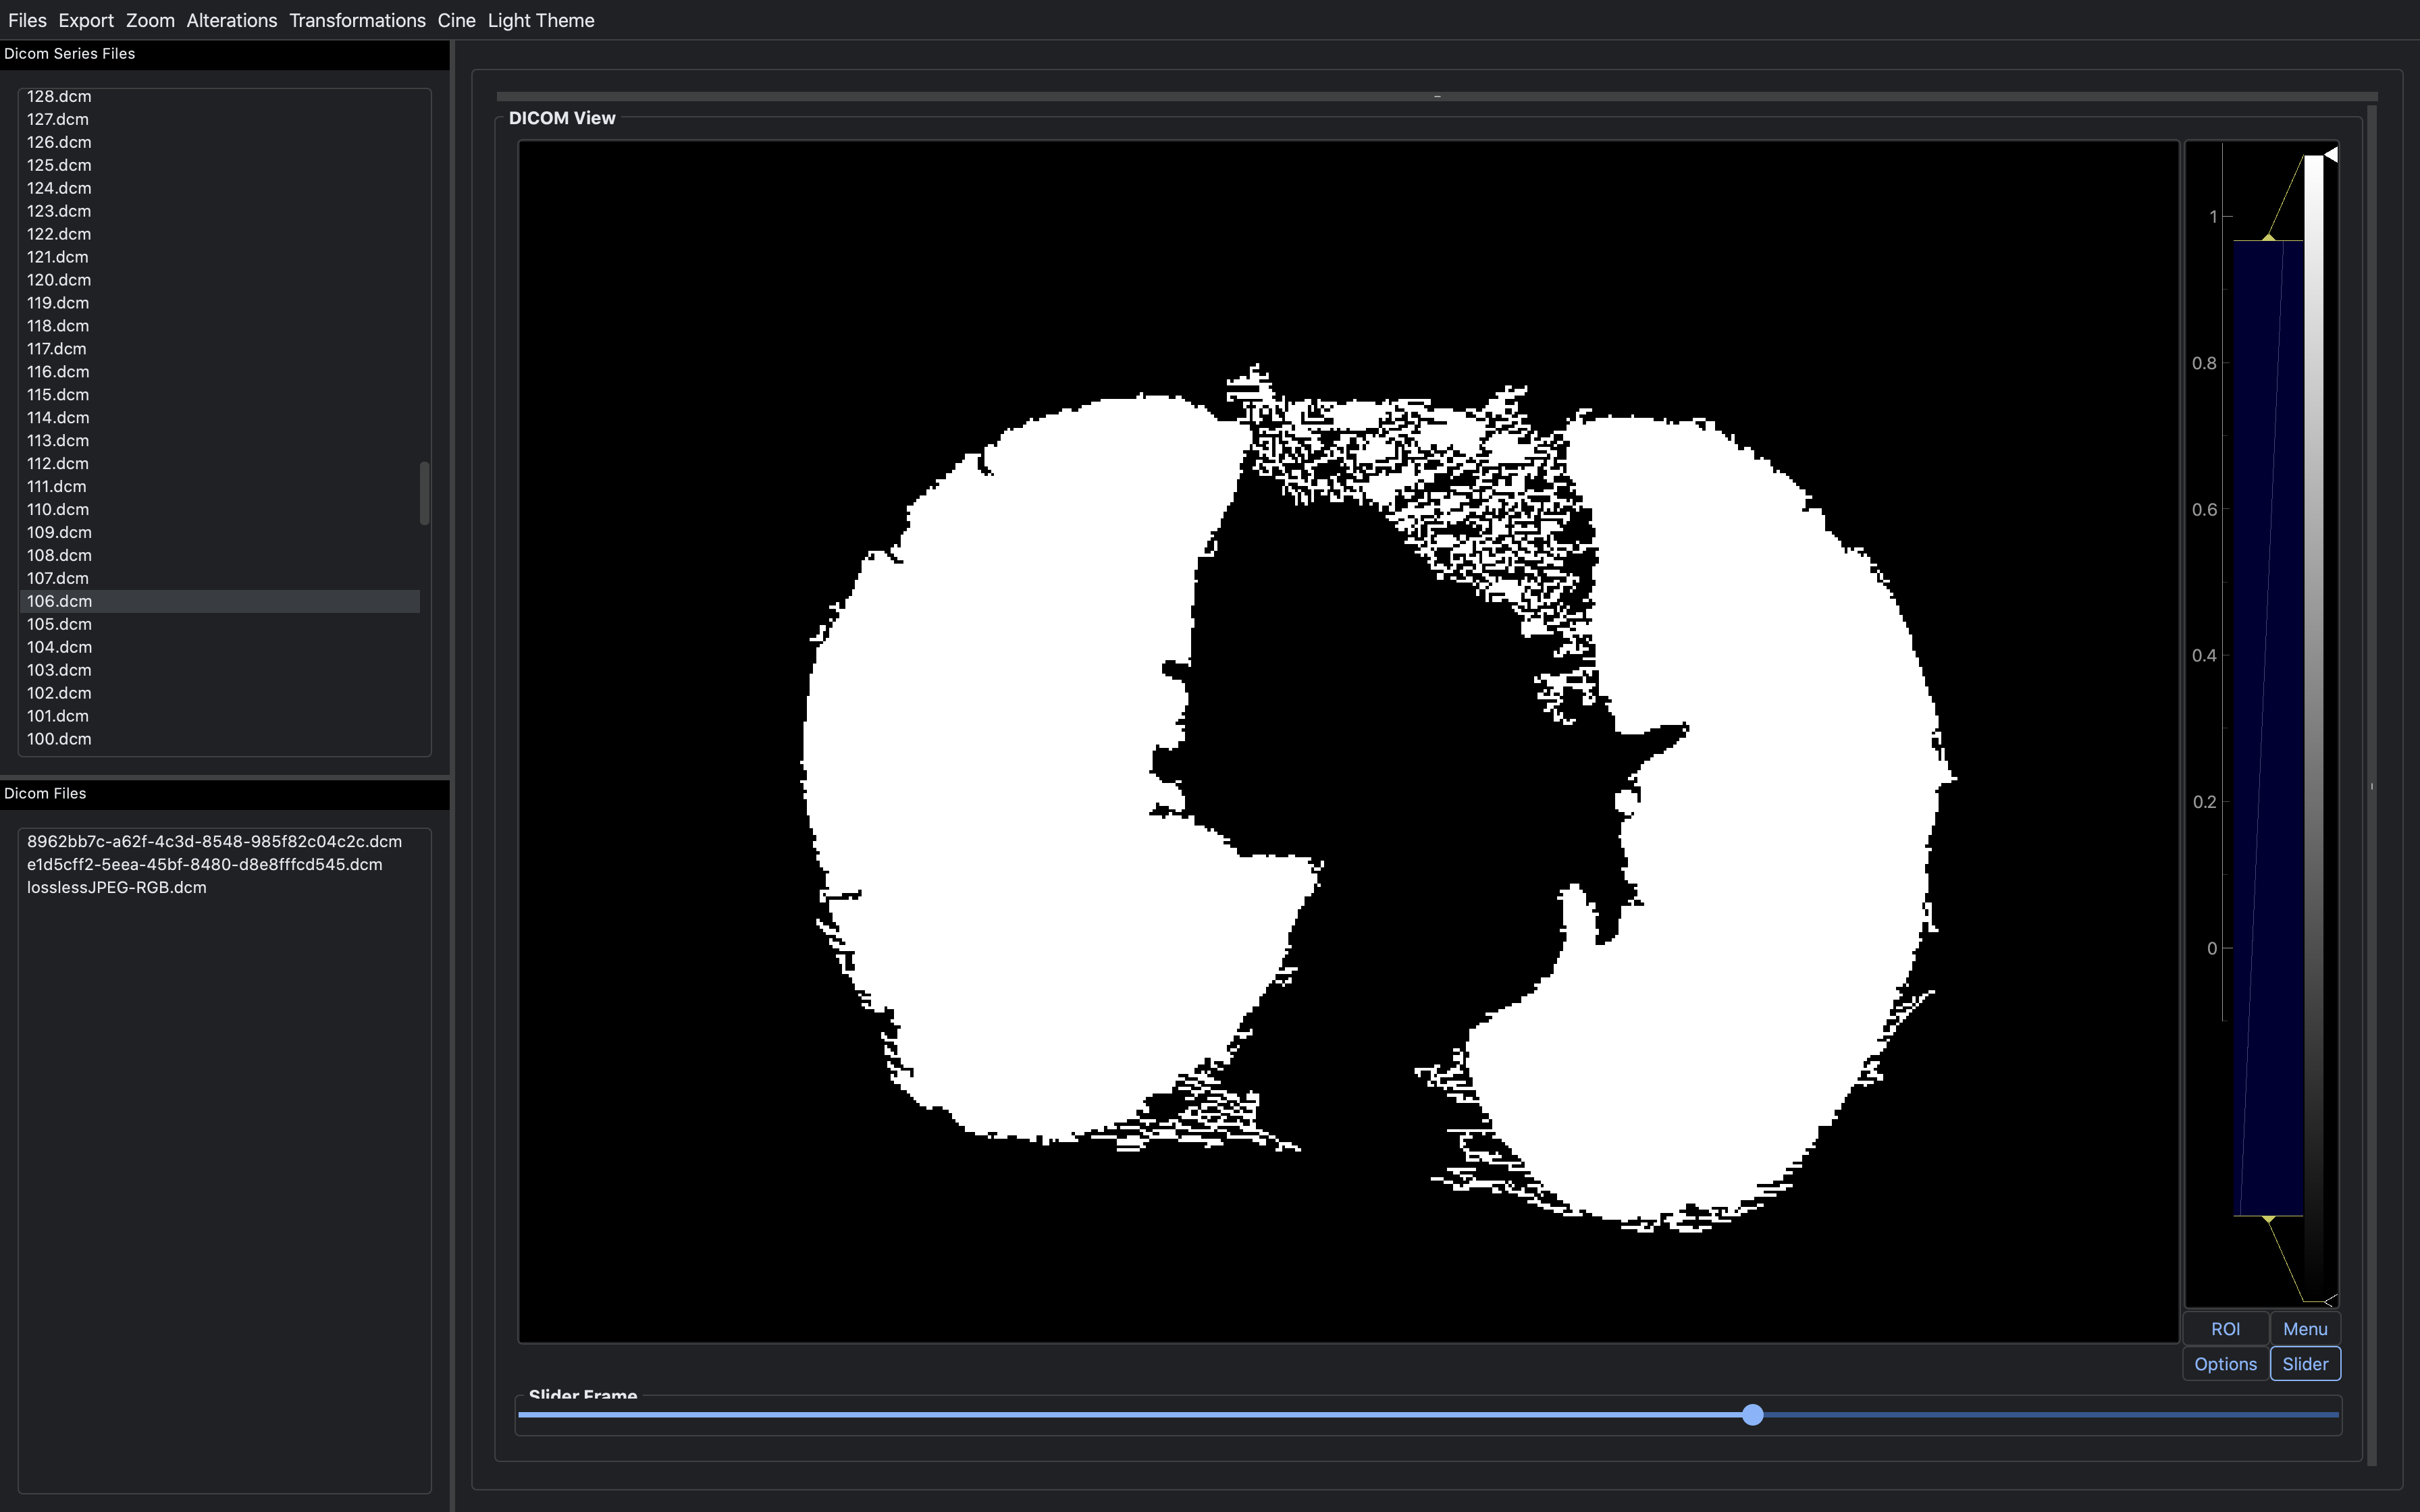
\includegraphics[width=\textwidth]{mask2.png}
            \caption[]%
            {{\small Lungs mask}}
            \label{fig:mean and std of net24}
        \end{subfigure}
        \vskip\baselineskip
        \begin{subfigure}[b]{0.475\textwidth}
            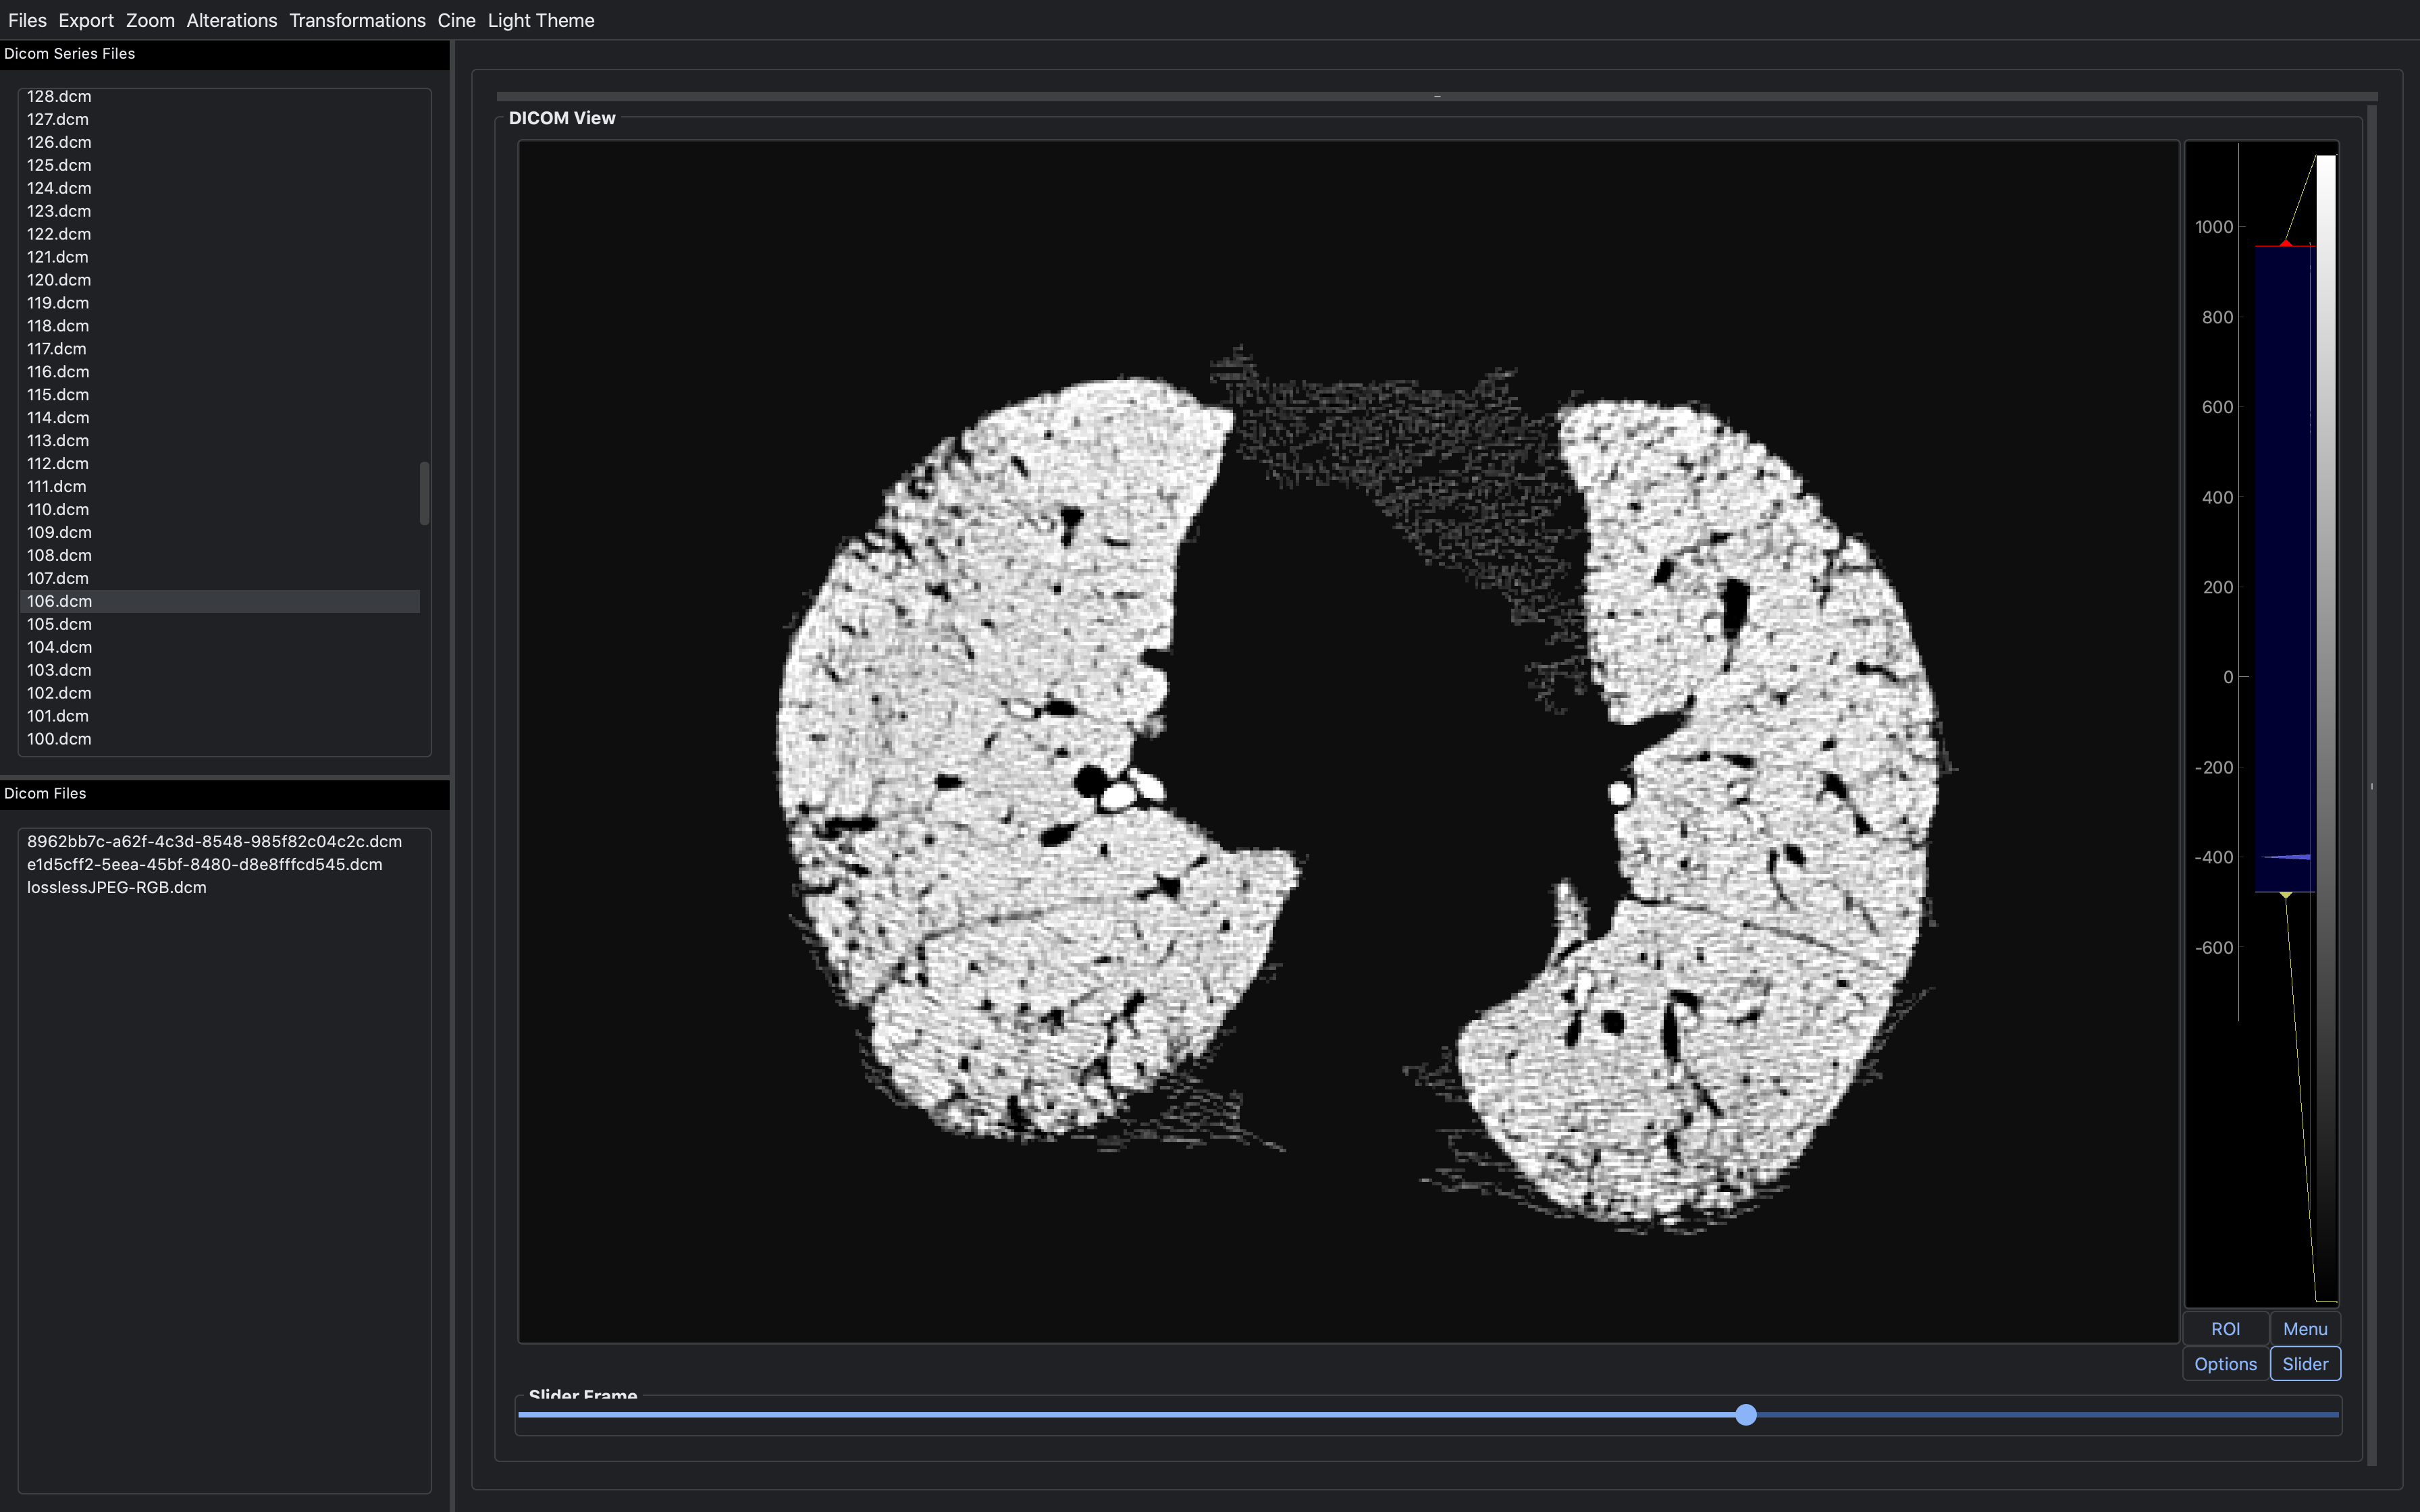
\includegraphics[width=\textwidth]{segmented.png}
            \caption[]%
            {{\small Segmented image with lungs mask}}
            \label{fig:mean and std of net34}
        \end{subfigure}
        \hfill
        \begin{subfigure}[b]{0.475\textwidth}
            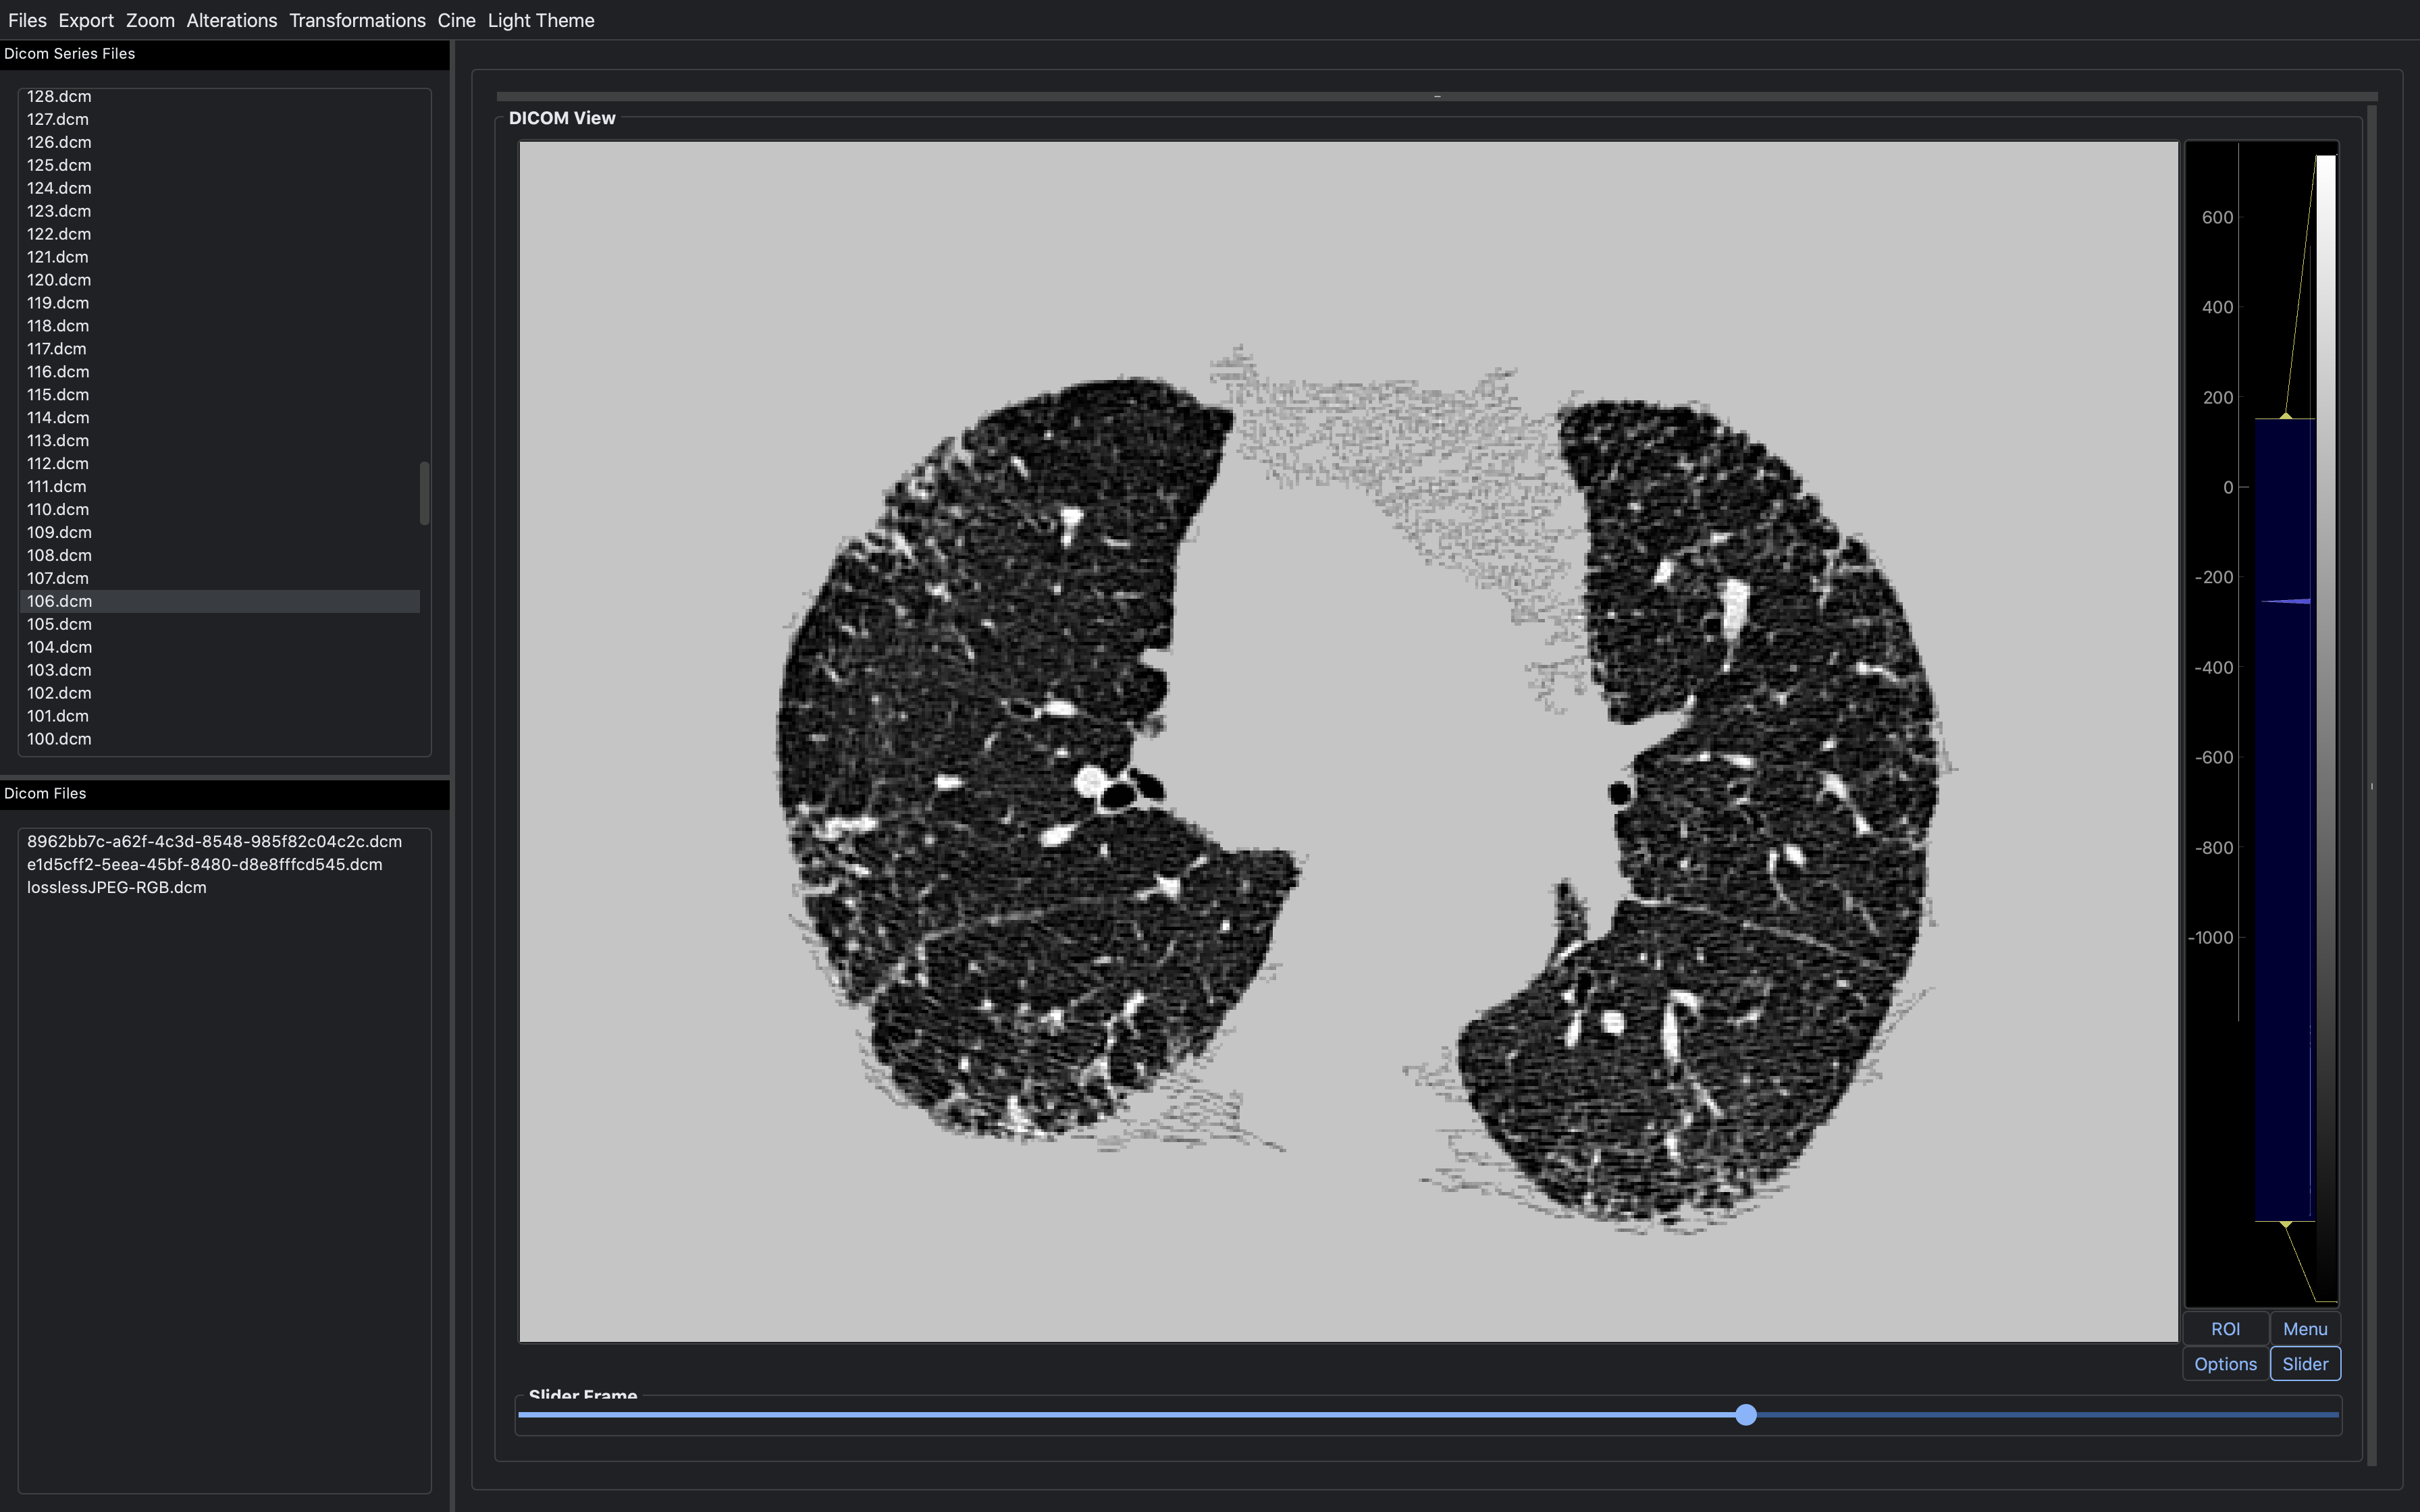
\includegraphics[width=\textwidth]{negative-segmented.png}
            \caption[]%
            {{\small Negative segmented image with lungs mask}}
            \label{fig:mean and std of net44}
        \end{subfigure}
        \caption[ The average and standard deviation of critical parameters ]
        {\small Example of image alteration of lungs acquisitions}
        \label{fig:mean and std of nets}
    \end{figure*}

\section{Image Alterations}

As stated in the abstract, even though the current state of the application is not oriented to image processing, some small experimental features are added to have a wider range of DicomViz usages. In particular, when working with lungs images, it is possible, through simple functions, to apply several modifications alone and combined together. An example of this is shown in Figure 4. These can be applied to currently viewed images through the homonymous menu items within the Menu "\textit{Alterations}", located in the "\textit{Menu Bar}". The provided alterations are:
\begin{itemize}
    \item \textbf{Negative image}: this consists in the application of the  \textit{NumPy}'s invert function on pixel data as array, which computes the bit-wise NOT of the underlying binary representation of the integers in the input array.

    \item \textbf{Lungs Mask}: this consists in the creation of a mask that covers the lungs, by determining the label of the air around the person, according to a  \textit{Household Units} treshold, whose value is not always the same and has to be tweaked. For this reason, a slider is provider to the user within the "\textit{Slider Frame}". Since during the air localization process both the external and internal lungs air is determined, to ensure an uniform mask only the largest air pocket (lungs' outer air) is considered.

    \item \textbf{Segmentation with lungs mask}: this consists in the segmentation of the lungs through the usage of the lungs mask function, but now considering lungs internal air. The mask is then applied to the original pixel data, together with lungs isolation from the rest of the image.
\end{itemize}


\section{Additional Implementation Details}

The DicomViz implementation follows an  \textit{Object Oriented} approach, whose choice was influenced by both  \textit{PyDicom} and  \textit{PyQt} packages, since their architecture relies on this programming paradigm. This promotes future maintenance and expansion.
The monkey patches were a sensible choice made to avoid the anti-pattern approach of modifying statically package code. This decision leads to various consequences. In the first place these run time alterations operate directly on library code, meaning that the natural future updates of the external source code will require consequent changes of the DicomViz code. Moreover these modifications allowed to provide significant and useful features. For example, as shown in Figure 5, the original  \textit{ImageView} provided only a portion of the buttons which are dynamically added. Another significant modification of such type is the insertion of additional colormaps, changing the available number of the histogram color maps from 12 to 174.

 \begin{figure}[h]
    \begin{minipage}{.49\columnwidth}
        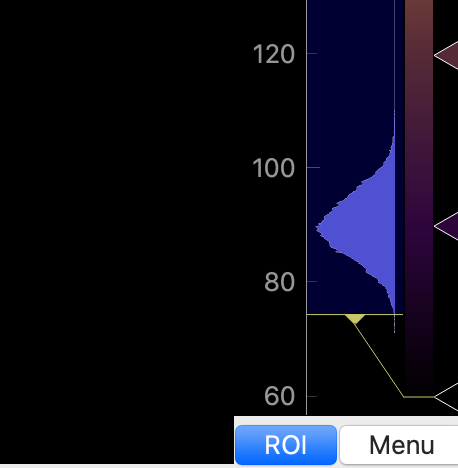
\includegraphics[width=\columnwidth]{orig.png}
        \subcaption{}
    \end{minipage}\hfill
    \begin{minipage}{.49\columnwidth}
        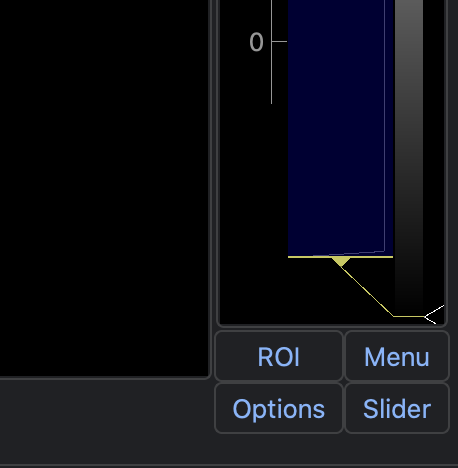
\includegraphics[width=\columnwidth]
        {but.png}
        \subcaption{}
    \end{minipage}
    \caption{(a) The screenshot on the left shows the original \\ structure of ImageView buttons, while (b) shows the implemented structure within DicomViz}
\end{figure}
In the initial steps of the implementation process several Python projects, both mantained and not, regarding Dicom standard, have been explored. Some of these helped to understand how to operate with imaging data, through  \textit{PyDicom} and  \textit{NumPy}. In particular, the open source  \textit{DicomBrowser}\cite{b4} project was highly helpful and some of its methods have been integrated into DicomViz, starting from the ones regarding data loading and processing to the ones regarding  \textit{PyQt} widgets usage.

\section{Limitations and Future Work}
The current state of the application works with some limitations mainly concerning performance, since the load of big series can lead to substantial background waiting time, due to the missing of a proper caching mechanism. This happens because during the load of a series from folder several time consuming operations are performed both to the whole sequence and to the single files, mainly regarding array calculations for image alterations, which could be executed subsequently when the user triggers the corresponding UI activation buttons, resulting in less slow downs.

Future works on DicomViz can concern additional features such as improved segmentation, lungs internal structures highlight, 3D visualization,
anonymization of Dicom patient data, internal storage system and support for Dicom file writing.

\section{Conclusions}

The application makes a proper usage of various solid and highly maintained libraries to provide a simple but effective visualizer intended to be an everyday tool to support the study of Dicom images.
The development process has allowed to understand the effectiveness and the simplicity of the Qt Framework and to understand the mechanisms behind the Dicom standard and the numerous consequent imaging applications.



\begin{thebibliography}{00}

\bibitem{b1}DICOM - \url{https://www.dicomstandard.org}
\bibitem{b2}RadiAnt - \url{https://www.radiantviewer.com}
\bibitem{b3}PostDICOM - \url{https://www.postdicom.com/it}
\bibitem{b4}DicomBrowser - \url{https://github.com/ericspod/DicomBrowser/tree/master/DicomBrowser}
\bibitem{b5}PyDicom \url{https://pydicom.github.io}
\bibitem{b6}NumPy - \url{https://numpy.org}
\bibitem{b7}QtDesigner - \url{https://doc.qt.io/qt-5/qtdesigner-manual.html}
\bibitem{b8}PyQt - \url{https://riverbankcomputing.com/software/pyqt/intro}
\bibitem{b9}PyQtGraph - \url{https://www.pyqtgraph.org}

\end{thebibliography}



\end{document}